\documentclass[12pt, letterpaper]{report}
\usepackage[utf8]{inputenc}
\usepackage{graphicx} % Required for inserting images
\usepackage{amsmath,amsfonts,amssymb}
\usepackage{algorithm}
\usepackage{algpseudocode}
\usepackage{cite}
\usepackage{url}
\usepackage{booktabs}
\usepackage{graphicx}
\usepackage{caption}
\usepackage[colorlinks]{hyperref}
\usepackage{xcolor}
\usepackage[margin=1in]{geometry}

\setlength{\parskip}{1em}
\setlength{\parindent}{0em}

\title{Efficient algorithms for infectious disease resource allocation model}
\author{Michael Ajao-olarinoye}
\date{April 2023}

\begin{document}

\maketitle

\section{new}
\begin{algorithm}
\caption{Physics-Informed Neural Network (PINN) Training for Epidemic Modeling}
\begin{algorithmic}[1]
\Require Training data tensors $S_{data}$, $I_{data}$, $R_{data}$, Time tensor $t_{data}$, Population $N$, Neural Network $NN$ with weights $w$ and biases $b$
\Ensure Preprocessed tensors on the same device
\State Initialize $NN$ with Xavier initialization for weights $w$ and biases $b$
\State Define early stopping criteria with patience and delta
\State Set learning rate $lr$ and regularization parameters $\lambda$, $p$

\For{each epoch up to $num\_epochs$}
    \State Compute predictions: $S_{pred}$, $I_{pred}$, $R_{pred} \gets NN(t_{data})$
    \State Compute time derivatives of $S_{pred}$, $I_{pred}$, $R_{pred}$ via autograd
    \State Calculate residuals using SIR model equations:
    \begin{align*}
    \frac{dS}{dt} & = -\beta \frac{S_{pred} I_{pred}}{N} \\
    \frac{dI}{dt} & = \beta \frac{S_{pred} I_{pred}}{N} - \gamma I_{pred} \\
    \frac{dR}{dt} & = \gamma I_{pred}
    \end{align*}
    \State Compute loss function components:
    \State $MSE_{SIR} \gets \frac{1}{q} \sum_{i=1}^{q} \left[ \left(S_{i} - S_{pred_i}\right)^2 + \left(I_{i} - I_{pred_i}\right)^2 + \left(R_{i} - R_{pred_i}\right)^2 \right]$
    \State $MSE_{residuals} \gets \frac{1}{q} \sum_{i=1}^{q} \left[ \left(\frac{dS_i}{dt} - \frac{dS_{pred_i}}{dt}\right)^2 + \left(\frac{dI_i}{dt} - \frac{dI_{pred_i}}{dt}\right)^2 + \left(\frac{dR_i}{dt} - \frac{dR_{pred_i}}{dt}\right)^2 \right]$
    \State $Loss \gets MSE_{SIR} + MSE_{residuals} + \lambda \cdot \text{Regularization}(NN)$
    \State Update $NN$ parameters via backpropagation and optimization step
    \State Adjust learning rate with learning rate scheduler if needed
    \State Check for early stopping, break if condition is met
\EndFor

\State \textbf{Output:} Trained PINN model $NN$
\end{algorithmic}
\end{algorithm}


\begin{algorithm}
\caption{Training of Physics-Informed Neural Network (PINN) for Epidemic Modeling}
\begin{algorithmic}[1]
\Require Training data tensors $\bm{S}_{data}$, $\bm{I}_{data}$, $\bm{R}_{data}$, time tensor $\bm{t}_{data}$, population size $N$, initial learning rate $lr$, regularization parameters $\lambda_{reg}$, $p_{reg}$, and number of epochs $num\_epochs$.
\Ensure All tensors are on the computational device, e.g., GPU.
\State Initialize PINN $NN$ with weights $\bm{w}$ and biases $\bm{b}$ using Xavier initialization.
\State Define EarlyStopping class with patience, delta, and verbose output.
\State Set up the Adam optimizer with learning rate $lr$ and weight decay.
\State Set up learning rate scheduler with reduction factor and patience.

\For{$epoch = 1$ to $num\_epochs$}
    \State Compute predictions $\bm{S}_{pred}$, $\bm{I}_{pred}$, $\bm{R}_{pred}$ from $NN(\bm{t}_{data})$.
    \State Compute gradients $\frac{d\bm{S}_{pred}}{dt}$, $\frac{d\bm{I}_{pred}}{dt}$, $\frac{d\bm{R}_{pred}}{dt}$ with respect to $\bm{t}_{data}$ using automatic differentiation.
    
    \State Define the SIR model's theoretical dynamics:
    \begin{align*}
    \frac{dS}{dt} & = -\beta \frac{S I}{N}, \\
    \frac{dI}{dt} & = \beta \frac{S I}{N} - \gamma I, \\
    \frac{dR}{dt} & = \gamma I.
    \end{align*}
    
    \State Compute the loss components:
    \begin{align*}
    MSE_{SIR} & = \frac{1}{q} \sum_{i=1}^{q} \left[ \left(\bm{S}_{i} - \bm{S}_{pred_i}\right)^2 + \left(\bm{I}_{i} - \bm{I}_{pred_i}\right)^2 + \left(\bm{R}_{i} - \bm{R}_{pred_i}\right)^2 \right], \\
    MSE_{residuals} & = \frac{1}{q} \sum_{i=1}^{q} \left[ \left(\frac{d\bm{S}_{pred_i}}{dt} + \beta \frac{\bm{S}_{pred_i} \bm{I}_{pred_i}}{N}\right)^2 + \left(\frac{d\bm{I}_{pred_i}}{dt} - \beta \frac{\bm{S}_{pred_i} \bm{I}_{pred_i}}{N} + \gamma \bm{I}_{pred_i}\right)^2 + \left(\frac{d\bm{R}_{pred_i}}{dt} - \gamma \bm{I}_{pred_i}\right)^2 \right].
    \end{align*}
    
    \State Compute regularization term (if L2 regularization is used):
    \begin{align*}
    Reg_{L2} = \lambda_{reg} \sum_{\bm{w}} \|\bm{w}\|^{p_{reg}}.
    \end{align*}
    
    \State Compute total loss:
    \begin{align*}
    Loss = MSE_{SIR} + MSE_{residuals} + Reg_{L2}.
    \end{align*}
    
    \State Perform backpropagation and update PINN parameters using the optimizer.
    \State Update learning rate with scheduler based on the validation loss.
    
    \If{EarlyStopping condition is met}
        \State \textbf{break}
    \EndIf
    
    \If{$(epoch + 1) \mod 100 = 0$ or $epoch = 0$}
        \State Log current epoch and loss for monitoring.
    \EndIf
\EndFor

\State \textbf{Output:} Trained PINN $NN$.
\end{algorithmic}
\end{algorithm}


\begin{algorithm}
\caption{Physics-Informed Neural Network (PINN) for SIR Dynamics}
\begin{algorithmic}[1]

\Require Training dataset $\mathcal{D} = \{(t_i, S_i, I_i, R_i)\}_{i=1}^{N}$, where $t_i$ denotes time, and $S_i$, $I_i$, $R_i$ represent susceptible, infected, and recovered individuals at time $t_i$, respectively.

\State \textbf{Data Preprocessing:}
\State Convert $\mathcal{D}$ into tensors: $\mathbf{S}, \mathbf{I}, \mathbf{R} \in \mathbb{R}^{N \times 1}$ and $\mathbf{t} \in \mathbb{R}^{N \times 1}$.

\State \textbf{Neural Network Architecture:}
\State Define a fully connected neural network $\mathcal{N}(\mathbf{t}; \theta)$ with input $\mathbf{t}$, parameters $\theta$, hidden layers, and Tanh activation functions. The network predicts $\hat{\mathbf{S}}, \hat{\mathbf{I}}, \hat{\mathbf{R}}$ at times $\mathbf{t}$.

\State \textbf{Loss Function:}
\State The loss function $\mathcal{L}(\theta)$ consists of two parts: the prediction loss and the differential equation loss.
\State Prediction loss: $\mathcal{L}_{\text{pred}} = \frac{1}{N}\sum_{i=1}^{N} \left( ||\hat{\mathbf{S}}_i - \mathbf{S}_i||^2 + ||\hat{\mathbf{I}}_i - \mathbf{I}_i||^2 + ||\hat{\mathbf{R}}_i - \mathbf{R}_i||^2 \right)$.
\State DE loss: Compute the gradients $\frac{d\hat{\mathbf{S}}}{dt}, \frac{d\hat{\mathbf{I}}}{dt}, \frac{d\hat{\mathbf{R}}}{dt}$ using automatic differentiation. Use these to define the SIR model's dynamics:
\begin{align*}
\frac{dS}{dt} &= -\beta \frac{SI}{N}, \\
\frac{dI}{dt} &= \beta \frac{SI}{N} - \gamma I, \\
\frac{dR}{dt} &= \gamma I.
\end{align*}
\State $\mathcal{L}_{\text{DE}} = \frac{1}{N}\sum_{i=1}^{N} \left( ||\frac{d\hat{\mathbf{S}}_i}{dt} + \beta \frac{\hat{\mathbf{S}}_i \hat{\mathbf{I}}_i}{N}||^2 + ||\frac{d\hat{\mathbf{I}}_i}{dt} - \beta \frac{\hat{\mathbf{S}}_i \hat{\mathbf{I}}_i}{N} + \gamma \hat{\mathbf{I}}_i||^2 + ||\frac{d\hat{\mathbf{R}}_i}{dt} - \gamma \hat{\mathbf{I}}_i||^2 \right)$.
\State Total loss: $\mathcal{L} = \mathcal{L}_{\text{pred}} + \mathcal{L}_{\text{DE}}$.

\State \textbf{Training:}
\State Use gradient descent to minimize $\mathcal{L}(\theta)$ with respect to $\theta$.
\State Apply early stopping based on validation loss to prevent overfitting.

\State \textbf{Evaluation:}
\State Evaluate the trained model $\mathcal{N}(\mathbf{t}; \theta^*)$ on test data to predict $\hat{\mathbf{S}}, \hat{\mathbf{I}}, \hat{\mathbf{R}}$.
\State Compare predictions with actual data to assess model performance.

\end{algorithmic}
\end{algorithm}



\begin{algorithm}
\caption{PINNs used to determine simultaneously the parameters of the neural network and the embedded SIR model.}
\begin{algorithmic}[1]

\Require Time points $t$, initial susceptible $S^0$, infected $I^0$, and recovered $R^0$ populations.
\State Randomly initialize weights $w$, biases $b$, and dynamics parameters $\beta, \gamma$;

\For{each epoch in epochs}
    \State The values of each compartment of the SIR model can be obtained from the forward propagation of the neural network with the input as $t$:
    \State $S, I, R = NN(t)$;
    
    \State Evaluate the composed loss function, including the data loss (with $s$ to be the number of observations in each compartment, thus the number of time points collected):
    \State $MSE_{SIR} = \frac{1}{s}\sum_{i=1}^{s} \left((S_i - S_i^0)^2 + (I_i - I_i^0)^2 + (R_i - R_i^0)^2\right)$, denoting the mismatch of the output of the neural network and observation data.
    
    \State Here the residual loss:
    \State $MSE_{residuals} = \frac{1}{q}\sum_{i=1}^{q} \left(\left|\left|\frac{dS_i}{dt_i} + \frac{\beta S_i I_i}{N}\right|\right|^2 + \left|\left|\frac{dI_i}{dt_i} - \frac{\beta S_i I_i}{N} + \gamma I_i\right|\right|^2 + \left|\left|\frac{dR_i}{dt_i} - \gamma I_i\right|\right|^2\right)$,
    \State stands for the sum of the residual errors for each compartment of the SIR model.
    
    \State Thus, the total loss function can be obtained:
    \State $Loss = MSE_{SIR} + MSE_{residuals}$;
    
    \State The Adam Optimizer toolkit in Pytorch is utilized to update the weights $w$ and biases $b$, as well as $\beta$ and $\gamma$ by minimizing the loss function.
\EndFor

\end{algorithmic}
\end{algorithm}

\begin{algorithm}
\caption{Training PINN for SIR Model}
\begin{algorithmic}[1]

\Require Time points $t$, initial susceptible $S_0$, infected $I_0$, recovered $R_0$, population $N$.
\State Randomly initialize neural network parameters $\theta$.

\For{each epoch}
    \State Obtain $S, I, R$ from neural network: $S, I, R = \mathcal{N}(t; \theta)$.
    \State Calculate data loss $MSE_{SIR}$:
    \State $MSE_{SIR} = \frac{1}{N}\sum_{i=1}^{N} ((S_i - S_{0i})^2 + (I_i - I_{0i})^2 + (R_i - R_{0i})^2)$.
    
    \State Compute residuals $\frac{dS}{dt}, \frac{dI}{dt}, \frac{dR}{dt}$ via autodiff.
    \State Calculate SIR model loss $MSE_{residuals}$:
    \State $MSE_{residuals} = \frac{1}{N}\sum_{i=1}^{N} \left( \left|\frac{dS_i}{dt} + \beta \frac{S_i I_i}{N}\right|^2 + \left|\frac{dI_i}{dt} - \beta \frac{S_i I_i}{N} + \gamma I_i\right|^2 + \left|\frac{dR_i}{dt} - \gamma I_i\right|^2 \right)$.
    
    \State Total loss $Loss = MSE_{SIR} + MSE_{residuals}$.
    \State Update $\theta$ using optimizer to minimize $Loss$.
    \State Implement early stopping if validation loss does not improve.
\EndFor

\end{algorithmic}
\end{algorithm}

\begin{algorithm}
\caption{Streamlined PINN Algorithm for SIR Model}
\begin{algorithmic}[1]

\Require Time points $t$, initial conditions $S_0, I_0, R_0$, total population $N$.
\State Randomly initialize network parameters $\theta$ and disease parameters $\beta, \gamma$.

\For{each epoch}
    \State Propagate $t$ through network to get $S, I, R = \mathcal{N}(t; \theta)$.
    
    \State Compute data fidelity loss $MSE_{SIR}$:
    \State $MSE_{SIR} = \frac{1}{N}\sum_{i=1}^{N} \big((S_i - S_{0i})^2 + (I_i - I_{0i})^2 + (R_i - R_{0i})^2\big)$.
    
    \State Derive SIR dynamics residuals via autodiff:
    \State $MSE_{residuals} = \frac{1}{N}\sum_{i=1}^{N} \left( \left|\frac{dS_i}{dt} + \beta \frac{S_i I_i}{N}\right|^2 + \left|\frac{dI_i}{dt} - \beta \frac{S_i I_i}{N} + \gamma I_i\right|^2 + \left|\frac{dR_i}{dt} - \gamma I_i\right|^2 \right)$.
    
    \State Define total loss $Loss = MSE_{SIR} + MSE_{residuals}$.
    \State Minimize $Loss$ to update $\theta$, $\beta$, and $\gamma$ with optimizer.
    \State Apply early stopping based on validation loss.
\EndFor

\end{algorithmic}
\end{algorithm}

\begin{algorithm}
\caption{Parameter Estimation for SEIRD Model via Differential Equation Learning}
\begin{algorithmic}[1]

\Require Time series data, population data, initial infected and death counts.

\State Normalize and partition data for model inputs.

\State Initialize model states $u(t_0) = [S_0, E_0, I_0, R_0, D_0]$.

\State Discretize time domain into $t_1, t_2, \ldots, t_n$.

\State Construct neural networks $NN_{\beta}(t;\theta_{\beta})$, $NN_{\gamma}(t;\theta_{\gamma})$, $NN_{\delta}(t;\theta_{\delta})$, $NN_{\alpha}(t;\theta_{\alpha})$ with parameters $\theta_{\beta}$, $\theta_{\gamma}$, $\theta_{\delta}$, $\theta_{\alpha}$.

\State Define the SEIRD differential equations with learned parameters:
\Function{SEIRD}{$\dot{u}, u, \theta, t$}
    \State $\beta(t), \gamma(t), \delta(t), \alpha(t) \gets |NN_{\beta}(t;\theta_{\beta})|, |NN_{\gamma}(t;\theta_{\gamma})|, |NN_{\delta}(t;\theta_{\delta})|, |NN_{\alpha}(t;\theta_{\alpha})|$
    \State $\dot{S}, \dot{E}, \dot{I}, \dot{R}, \dot{D} \gets \text{transitions based on SEIRD dynamics and } \beta(t), \gamma(t), \delta(t), \alpha(t)$
\EndFunction

\State Formulate the initial value problem (IVP) using $u(t_0)$ and SEIRD dynamics.

\State Define loss function $\mathcal{L}(\theta)$ combining prediction errors and parameter trajectory regularizations.

\State Minimize $\mathcal{L}(\theta)$ using gradient-based optimization with callbacks to monitor convergence.

\State Evaluate model fit with metrics such as MSE, MAE, MAPE, RMSE.

\end{algorithmic}
\end{algorithm}

The SIR model is described by the following set of differential equations:
\begin{align}
\frac{dS}{dt} &= -\beta \frac{SI}{N}, \\
\frac{dI}{dt} &= \beta \frac{SI}{N} - \gamma I, \\
\frac{dR}{dt} &= \gamma I,
\end{align}
where $S$ is the number of susceptible individuals, $I$ is the number of infectious individuals, $R$ is the number of recovered individuals, and $N$ is the total population.
\begin{tabular}{ll}
\toprule
\textbf{Parameter} & \textbf{Definition} \\
\midrule
$\beta$ & Transmission rate \\
$\gamma$ & Recovery rate \\
\bottomrule
\end{tabular}
The SEIRD model extends the SIR model by including compartments for exposed (E) and dead (D) individuals:
\begin{align}
\frac{dS}{dt} &= -\beta \frac{SI}{N}, \\
\frac{dE}{dt} &= \beta \frac{SI}{N} - \delta E, \\
\frac{dI}{dt} &= \delta E - (\gamma + \alpha) I, \\
\frac{dR}{dt} &= \gamma I, \\
\frac{dD}{dt} &= \alpha I,
\end{align}
where $E$ represents the exposed individuals who are infected but not yet infectious, and $D$ represents the deceased individuals.



\begin{tabular}{ll}
\toprule
\textbf{Parameter} & \textbf{Definition} \\
\midrule
$\beta$ & Transmission rate \\
$\delta$ & Rate at which exposed individuals become infectious \\
$\gamma$ & Recovery rate \\
$\alpha$ & Mortality rate \\
\bottomrule
\end{tabular}

\begin{figure*}[ht]
    \centering
    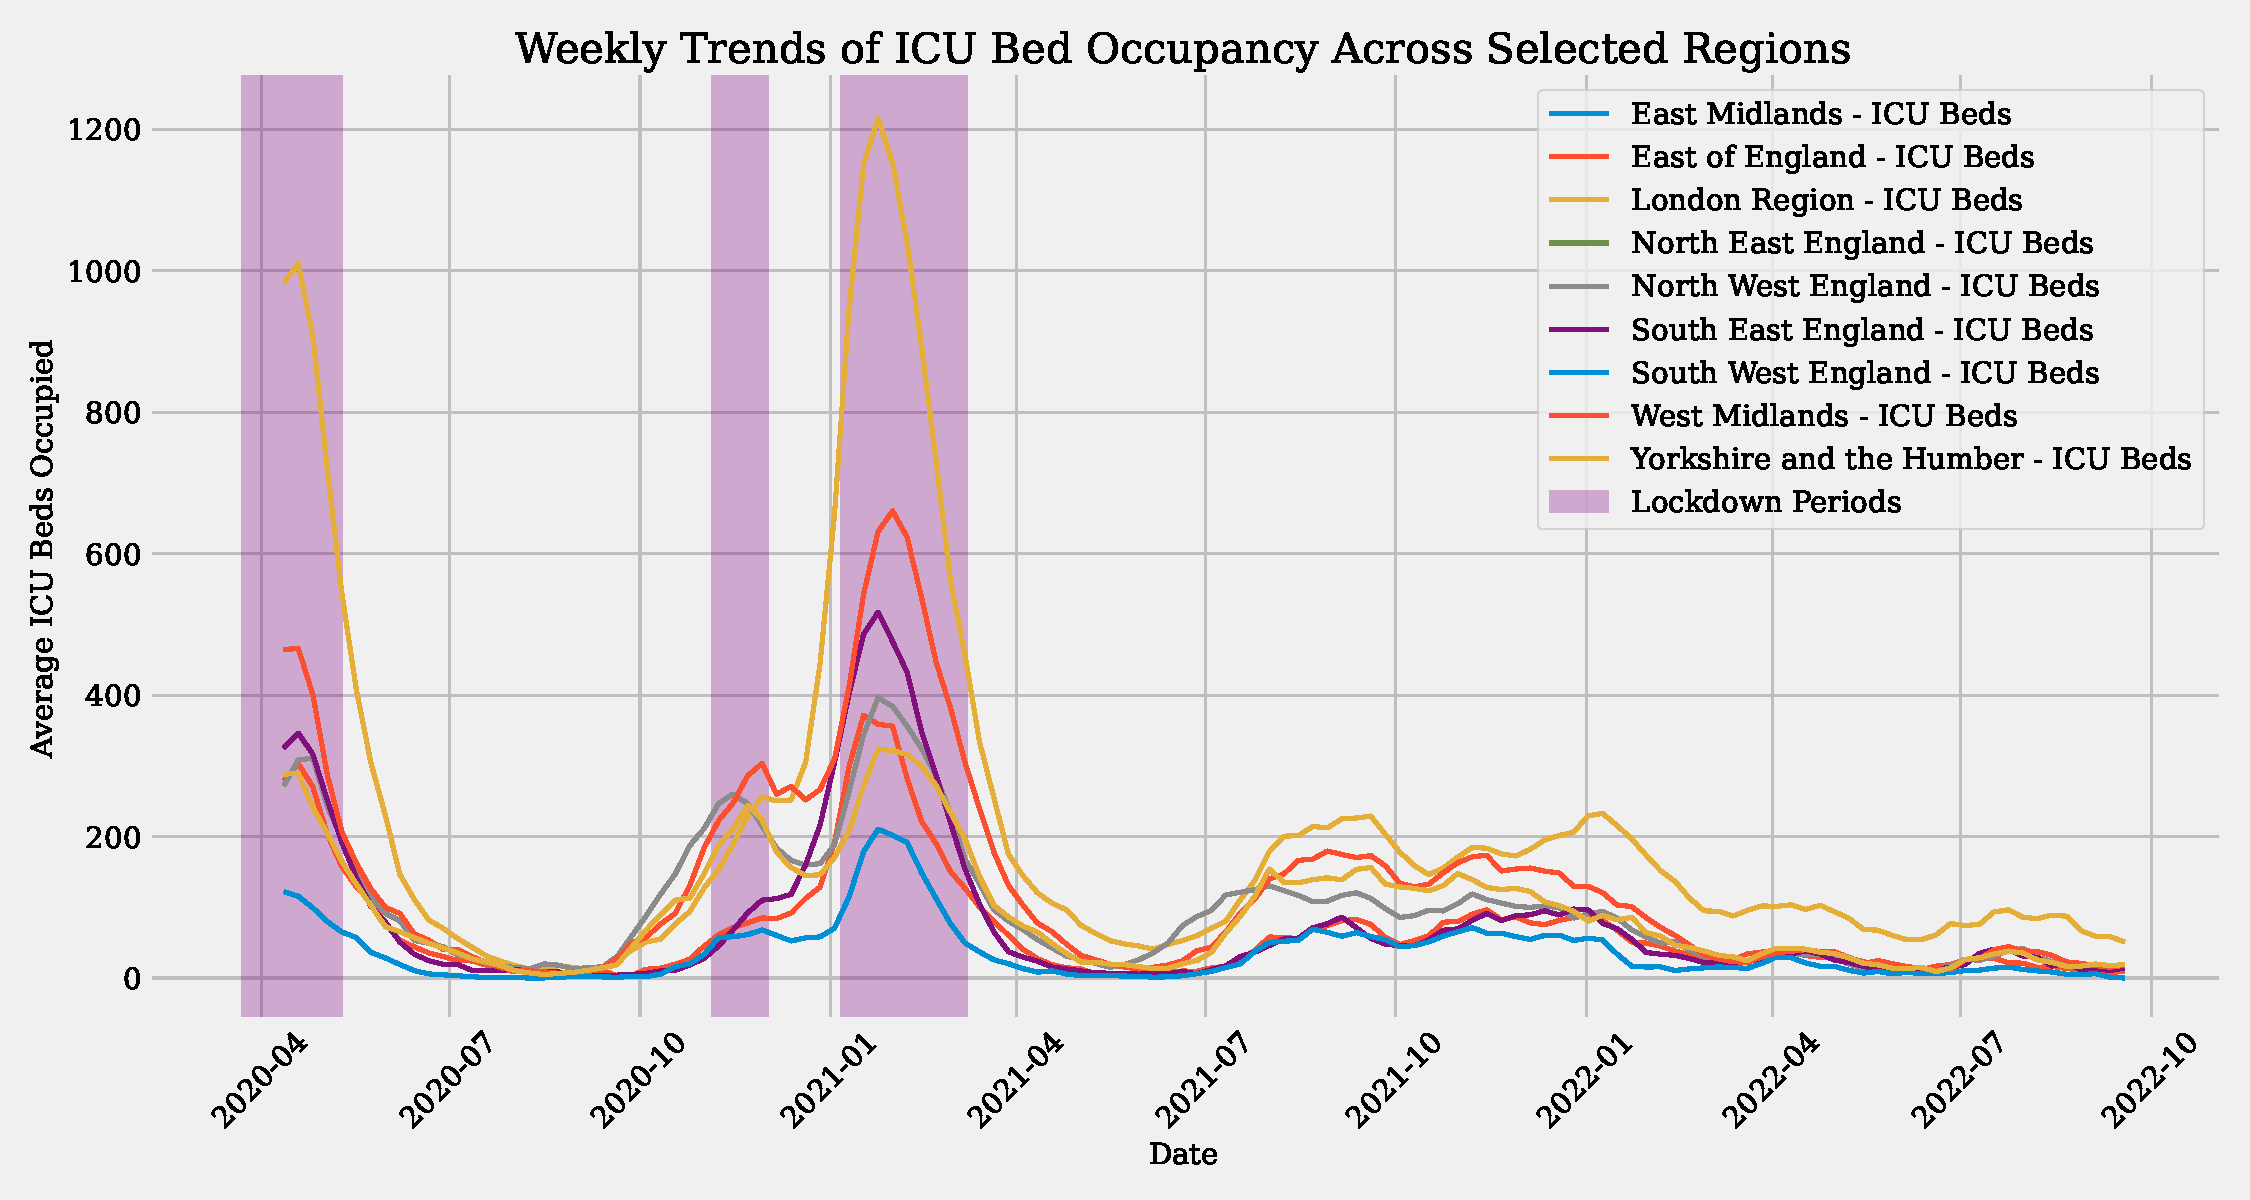
\includegraphics[width=0.8\textwidth]{"images/weekly_icu_beds_occupancy.pdf"}
    \caption{weekly ICU bed occupancy across NHS regions.}
    \label{fig:ICU_beds_occupancy}
\end{figure*}


\begin{figure*}[ht]
    \centering
    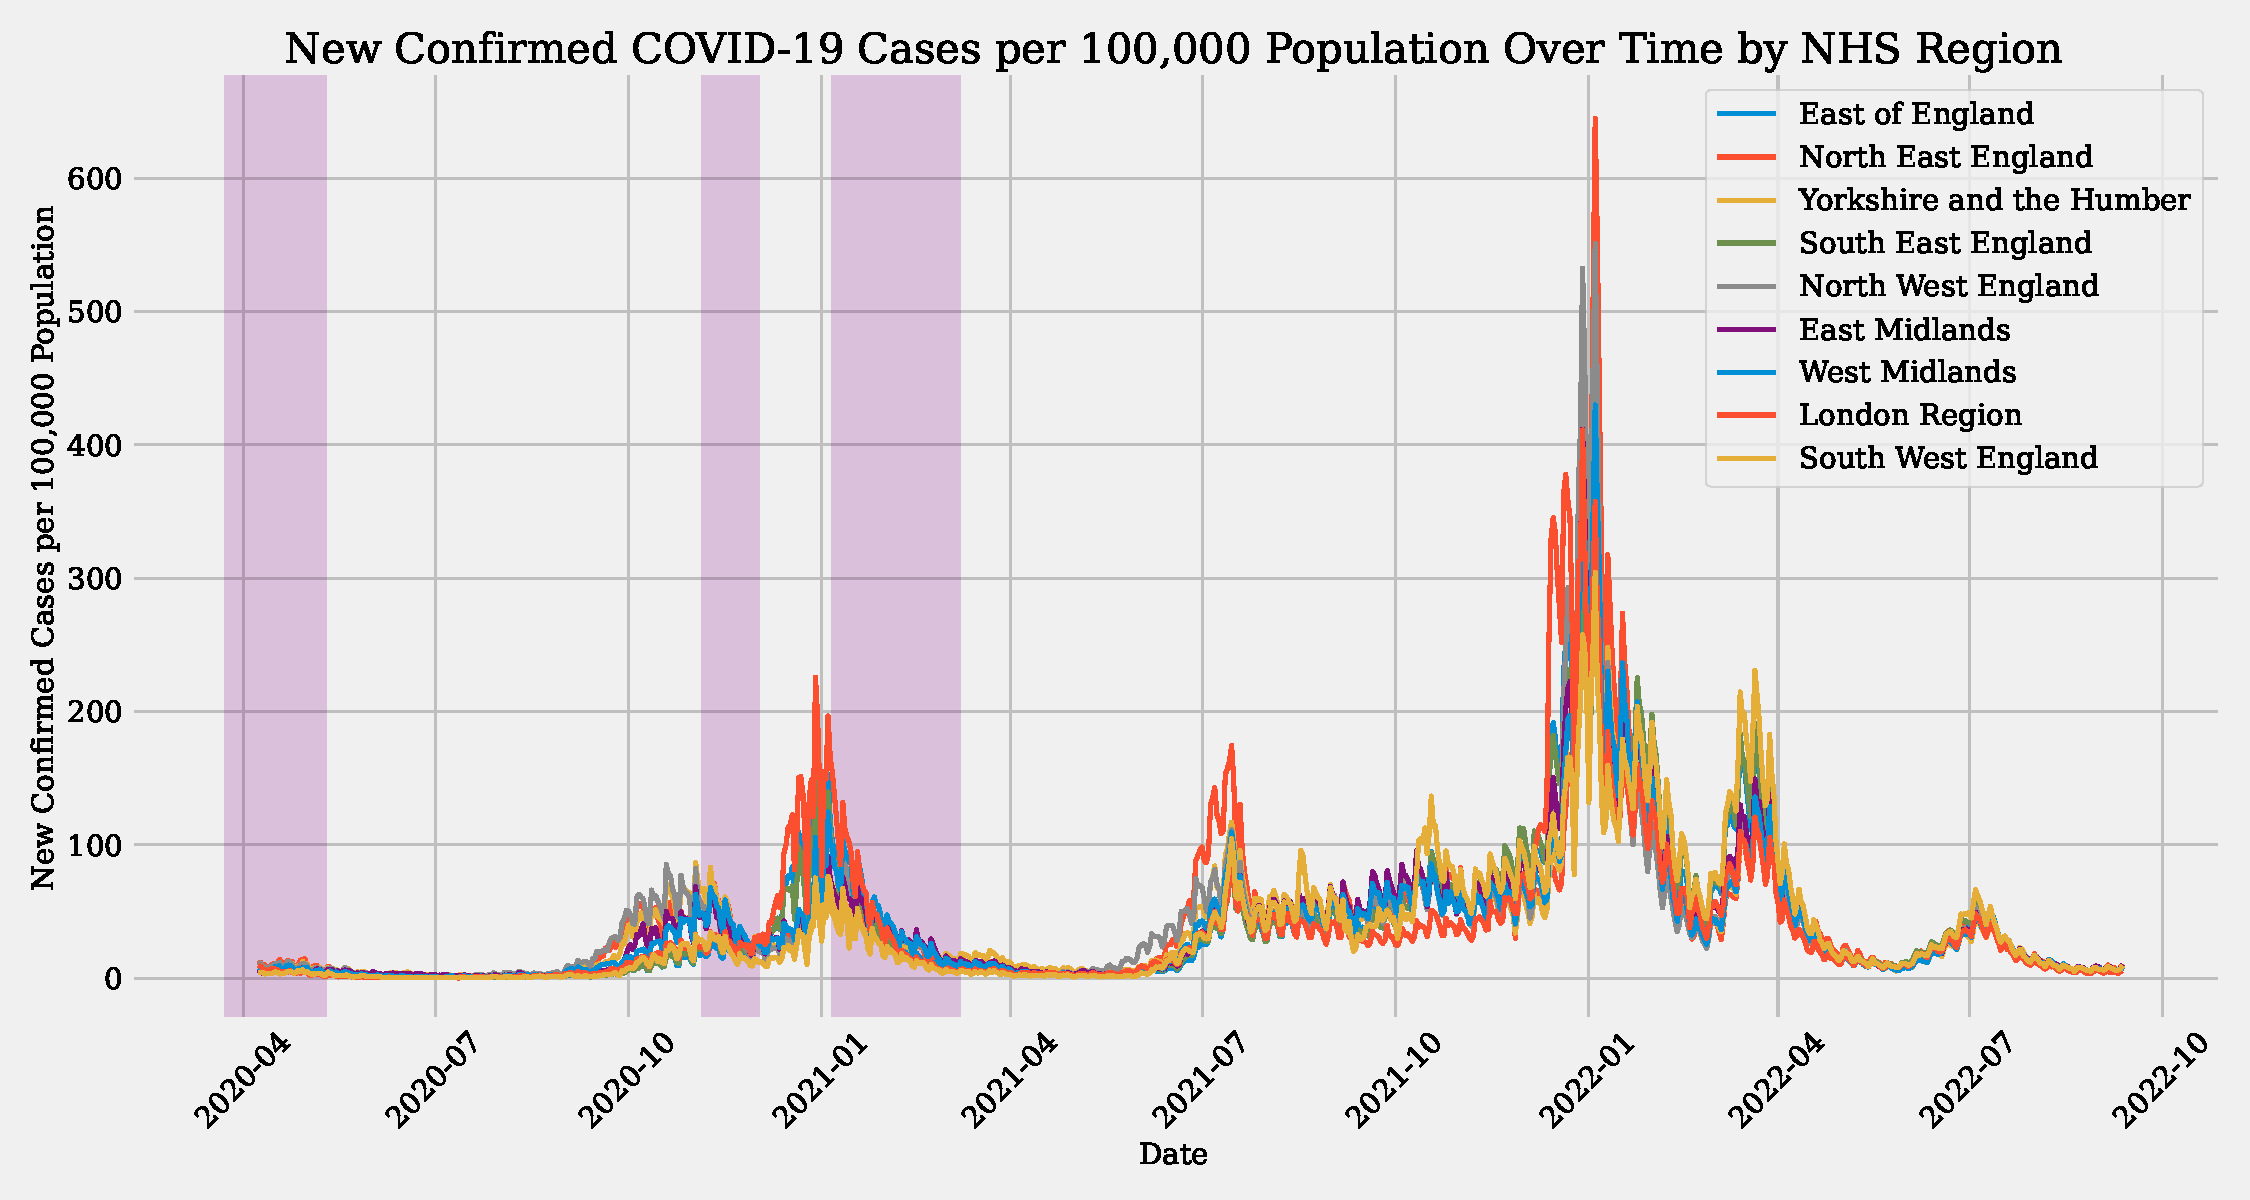
\includegraphics[width=0.8\textwidth]{"images/new_confirmed_per_100k.pdf"}
    \caption{new confirmed COVID-19 cases per 100k people overtime by NHS regions.}
    \label{fig:new_confirmed_per_100k}
\end{figure*}

\begin{figure*}[ht]
    \centering
    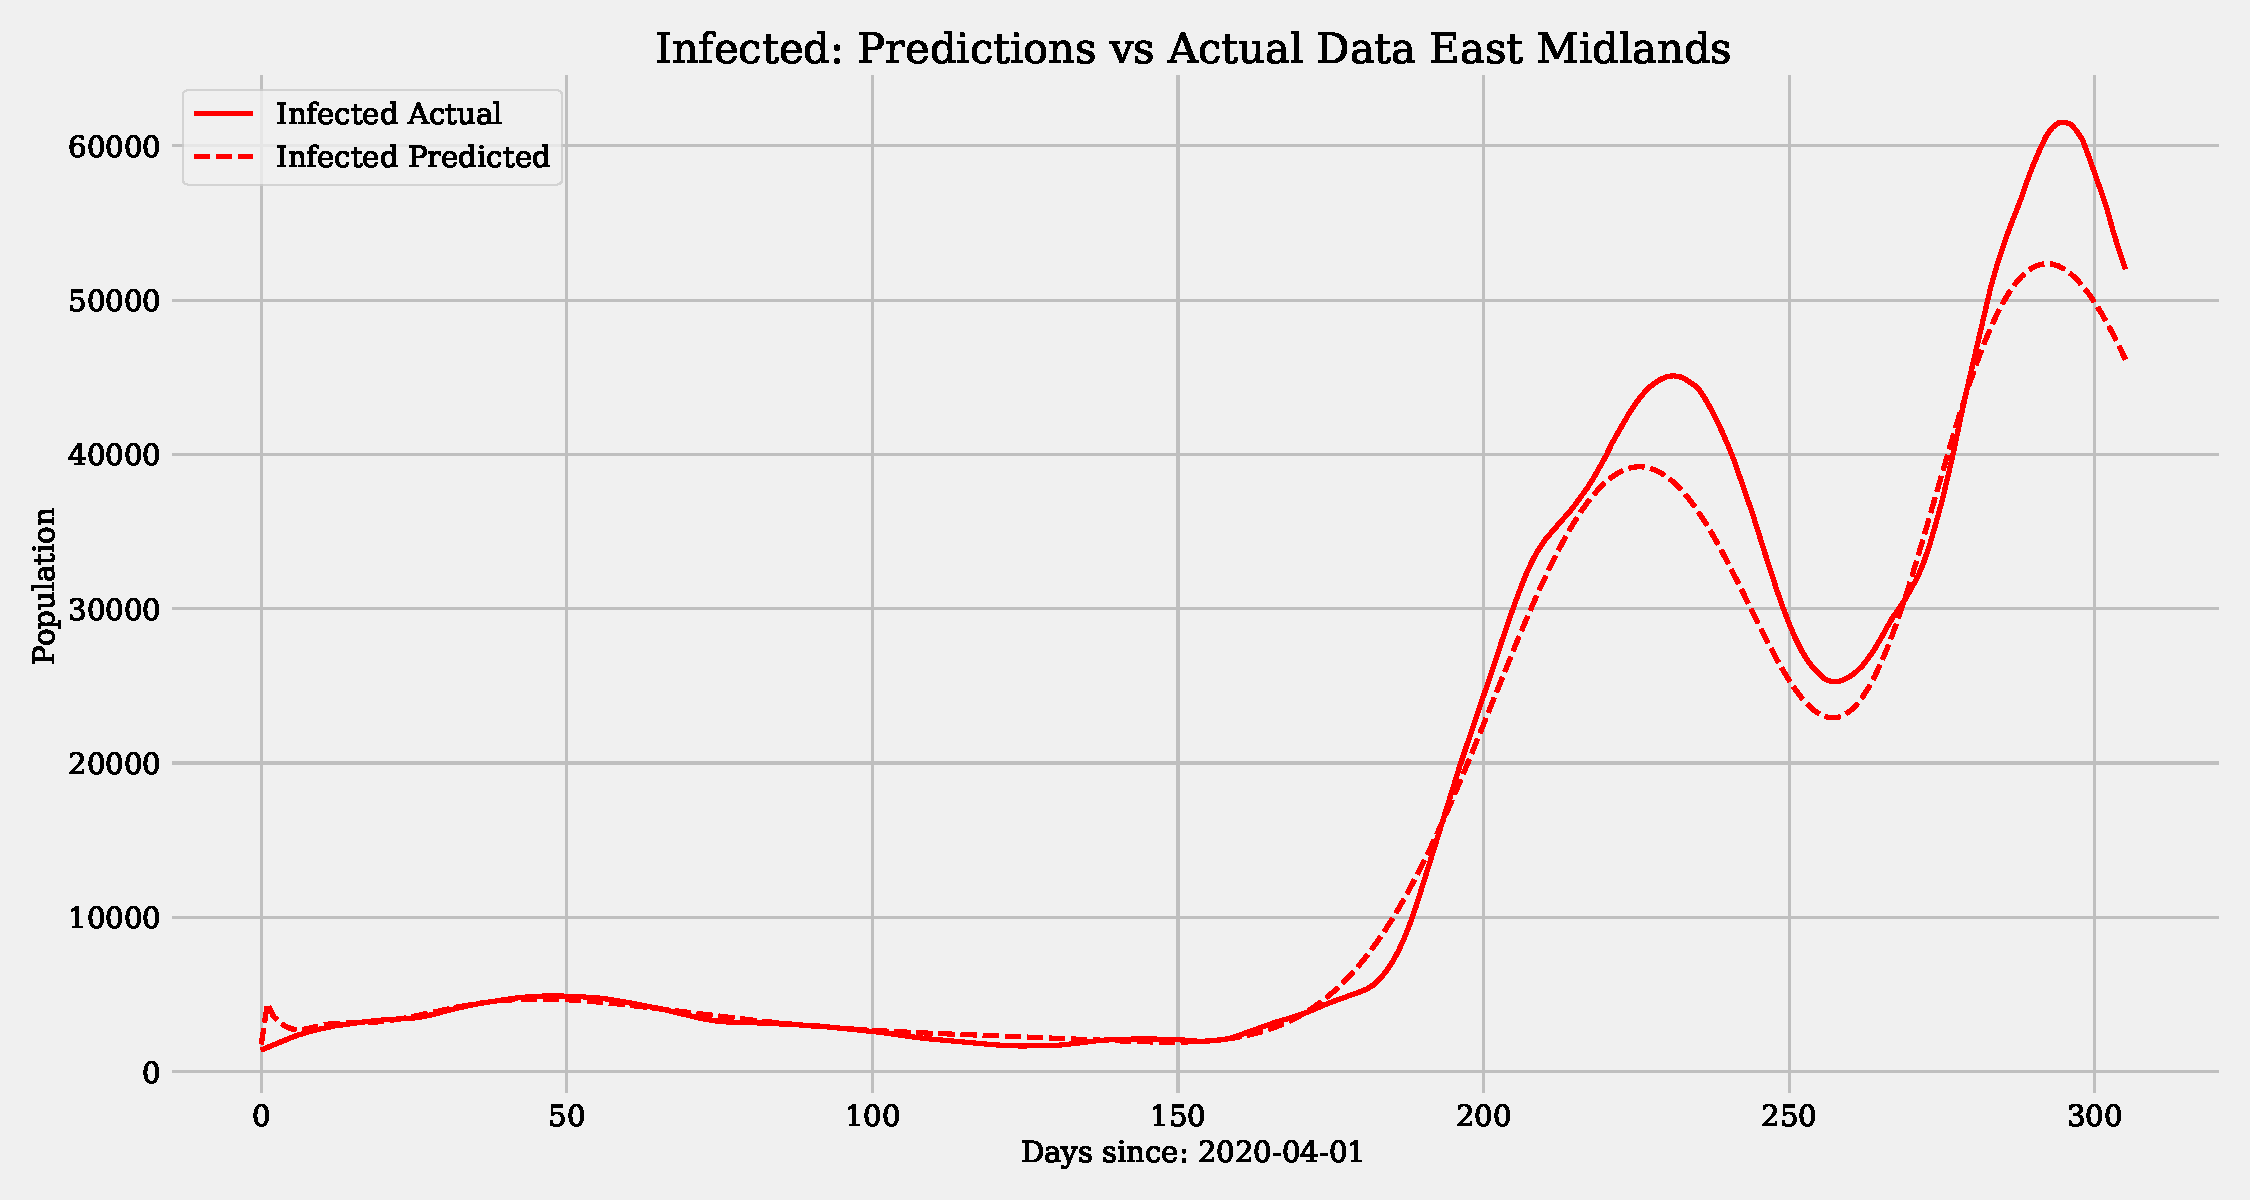
\includegraphics[width=0.8\textwidth]{images/pinn/I_predictions_East Midlands.pdf}
    \caption{Predicted number of infectious individuals in the East Midlands region.}
    \label{fig:I_predictions_East_Midlands}
\end{figure*}

\begin{figure*}[ht]
    \centering
    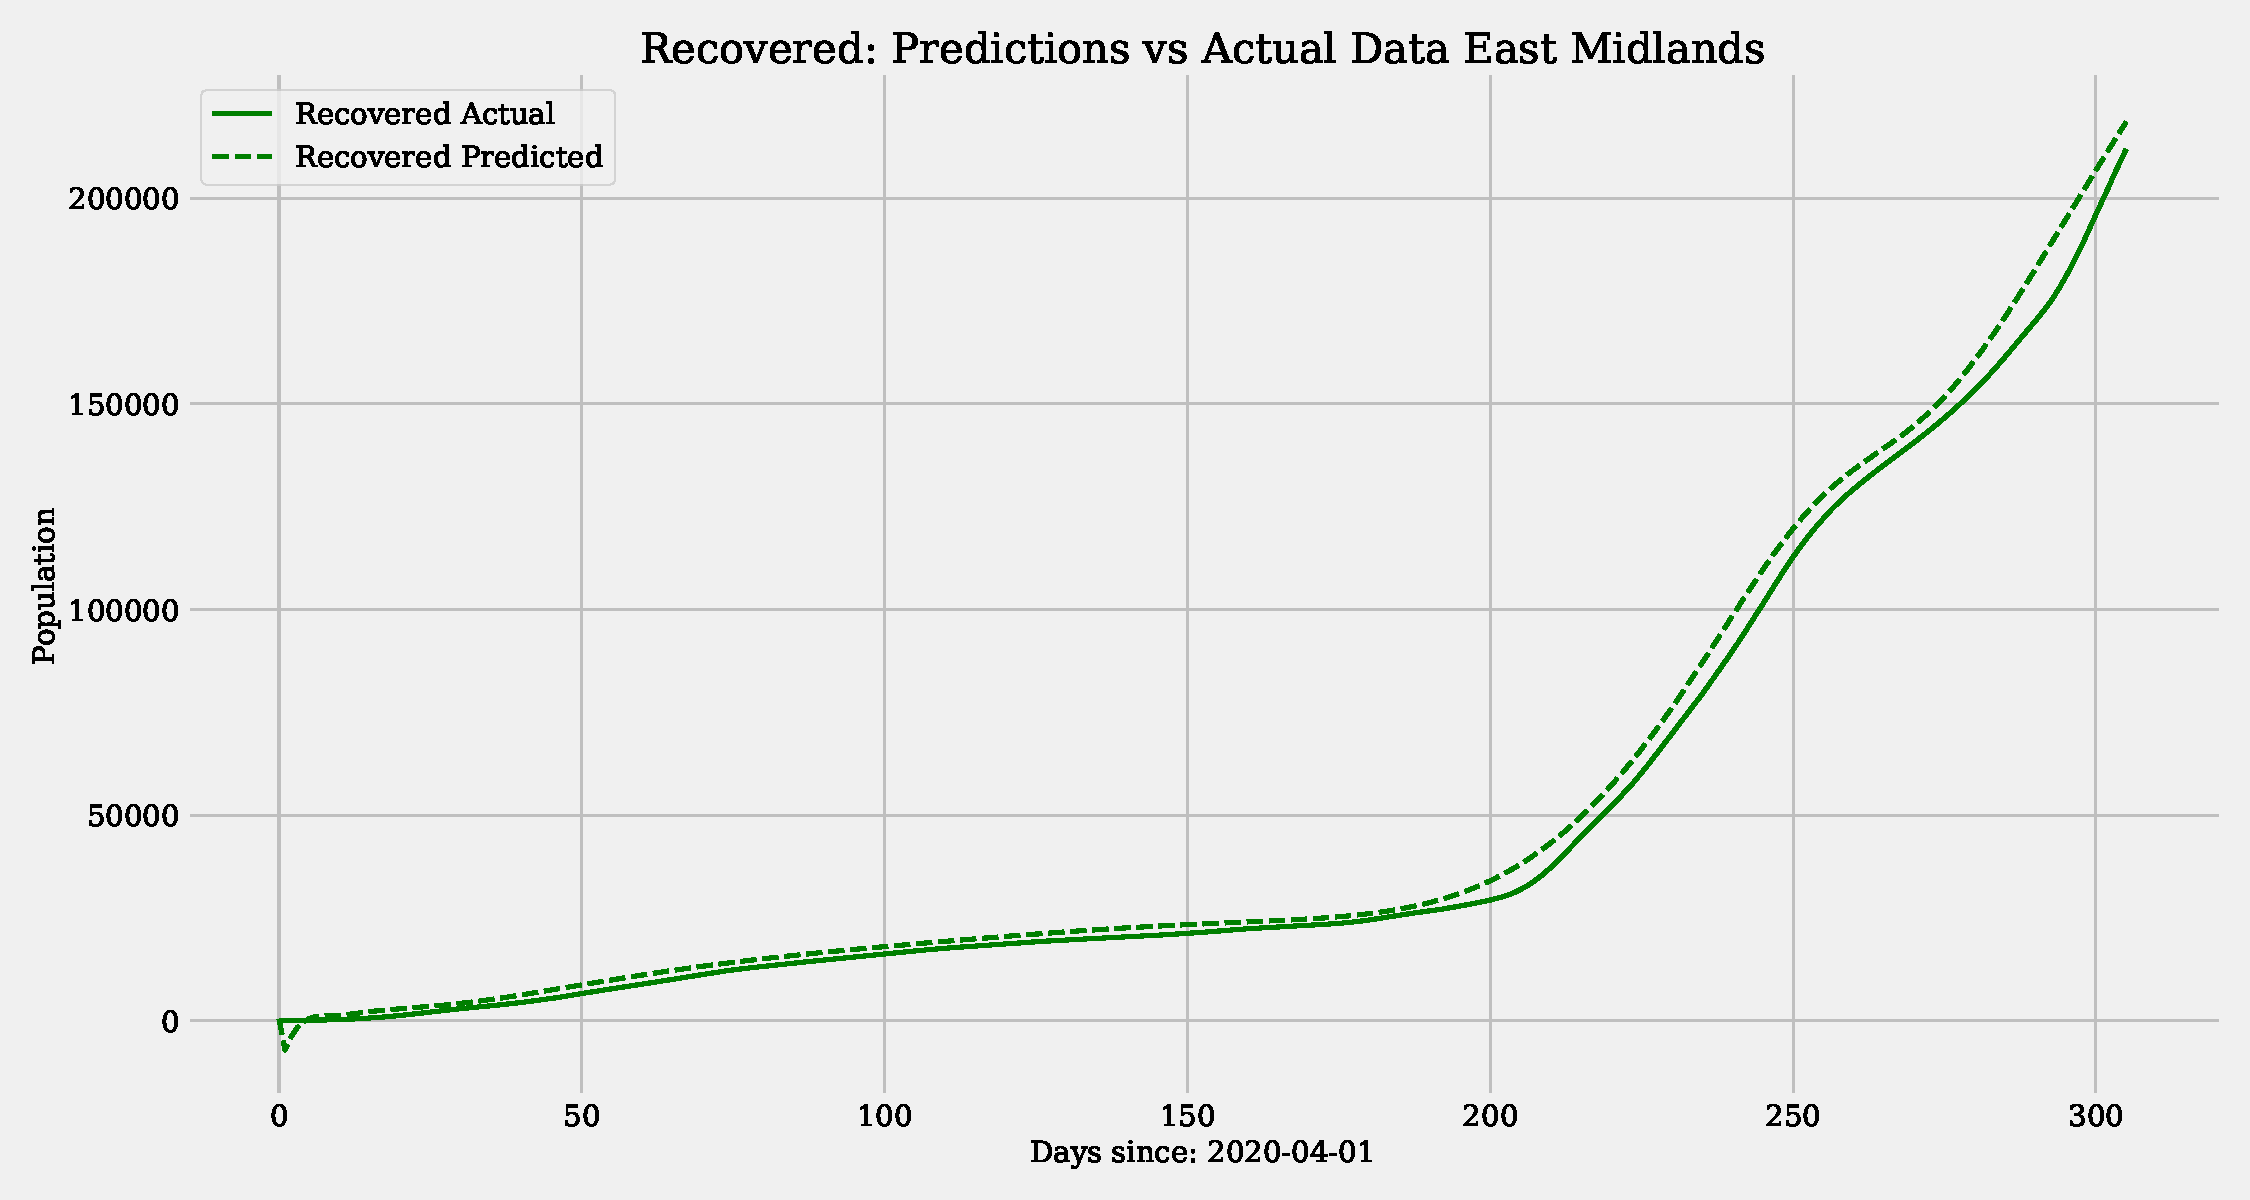
\includegraphics[width=0.8\textwidth]{images/pinn/R_predictions_East Midlands.pdf}
    \caption{Predicted number of recovered individuals in the East Midlands region.}
    \label{fig:R_predictions_East_Midlands}
\end{figure*}

\begin{figure*}[ht]
    \centering
    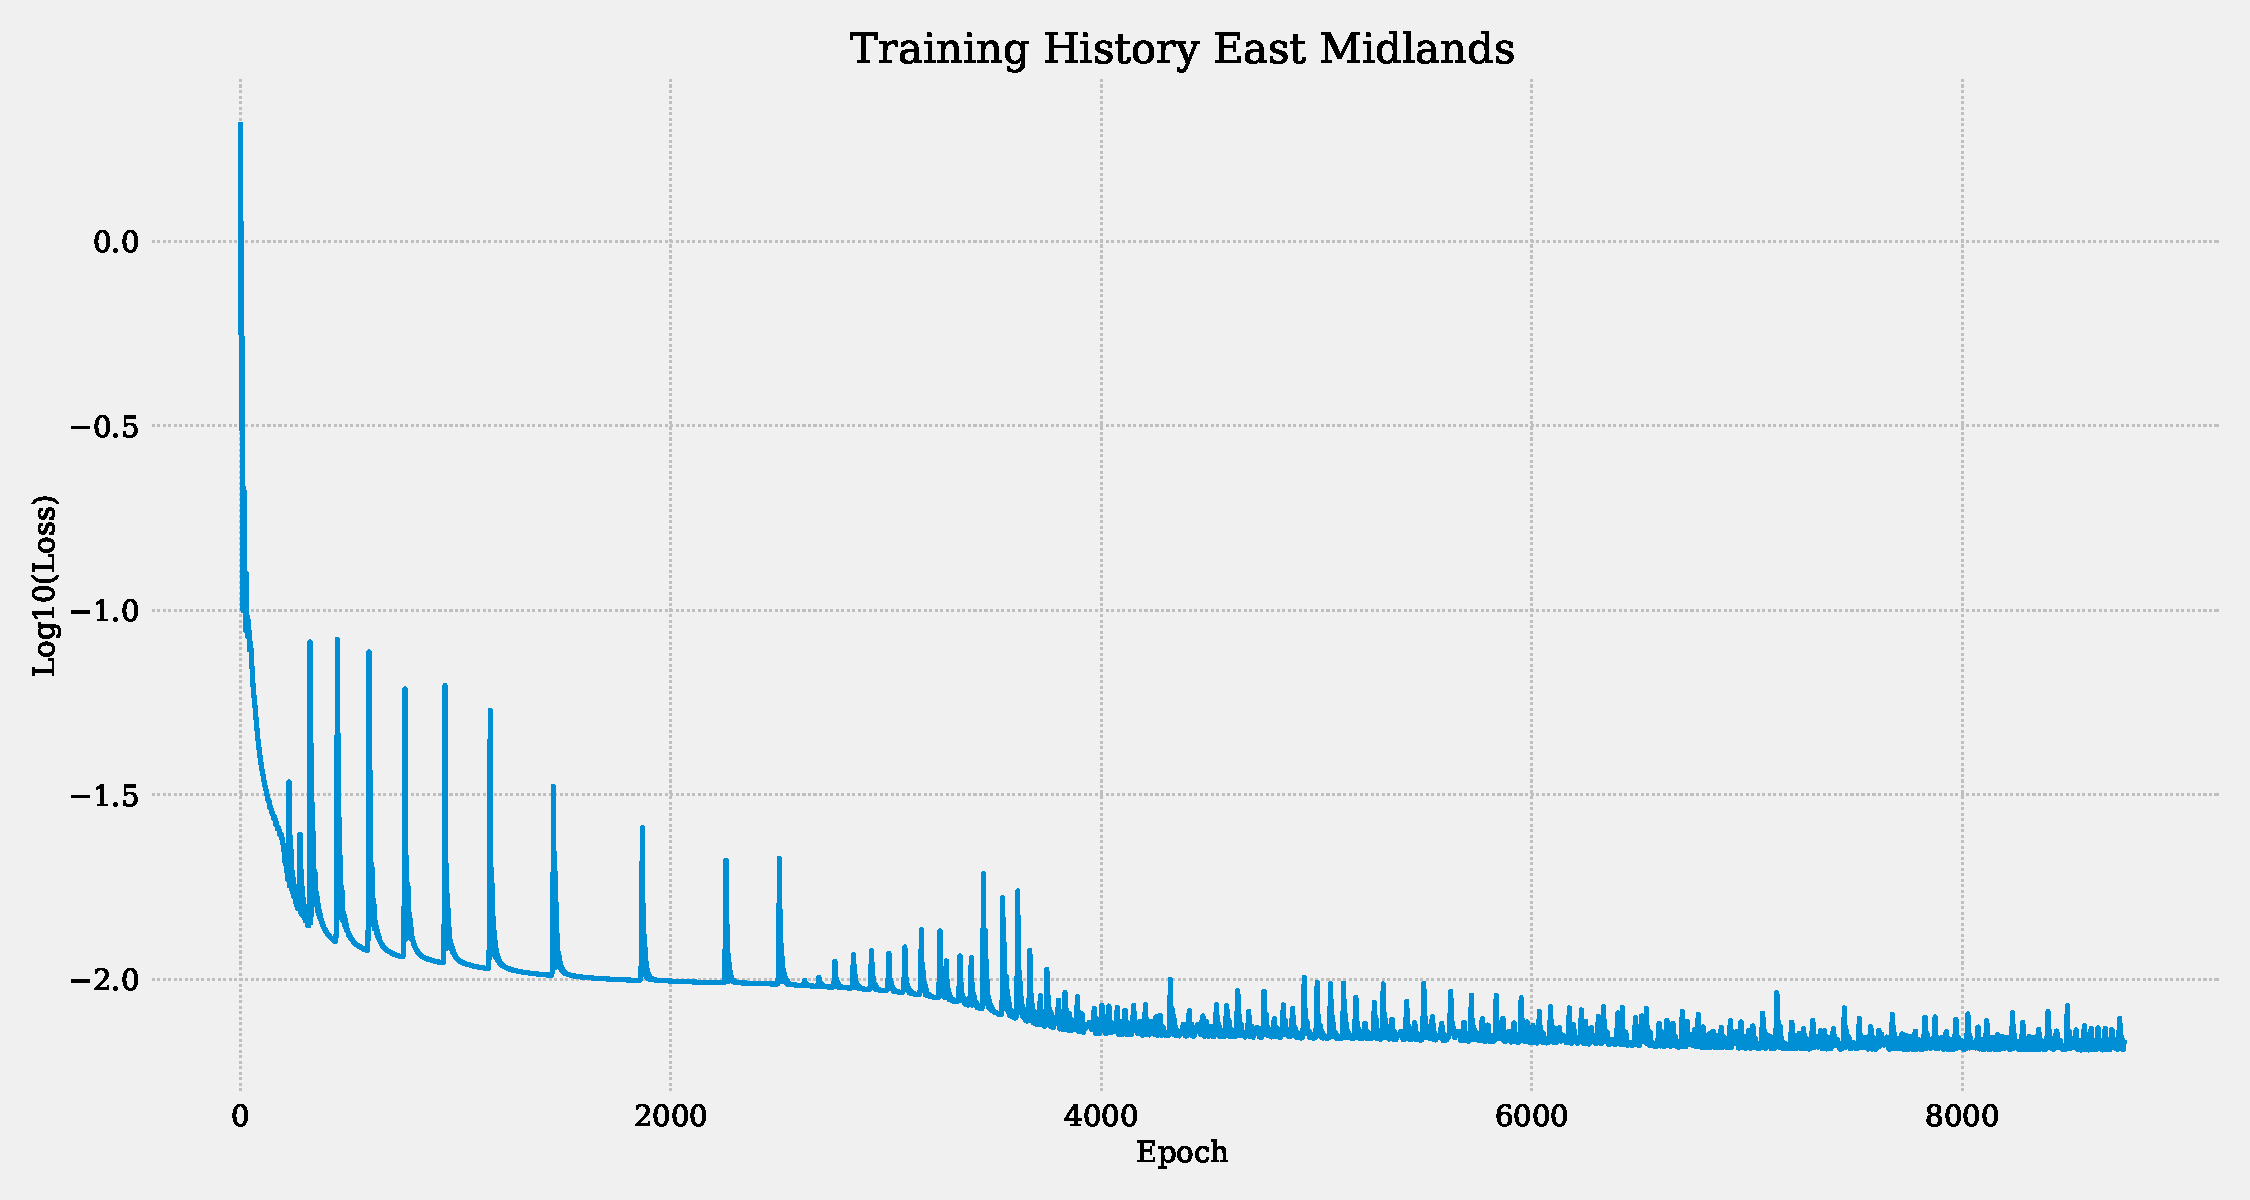
\includegraphics[width=0.8\textwidth]{images/pinn/Training_History_East Midlands.pdf}
    \caption{Training history of the PINN model for the East Midlands region.}
    \label{fig:Training_History_East_Midlands}
\end{figure*}

\begin{figure*}[ht]
    \centering
    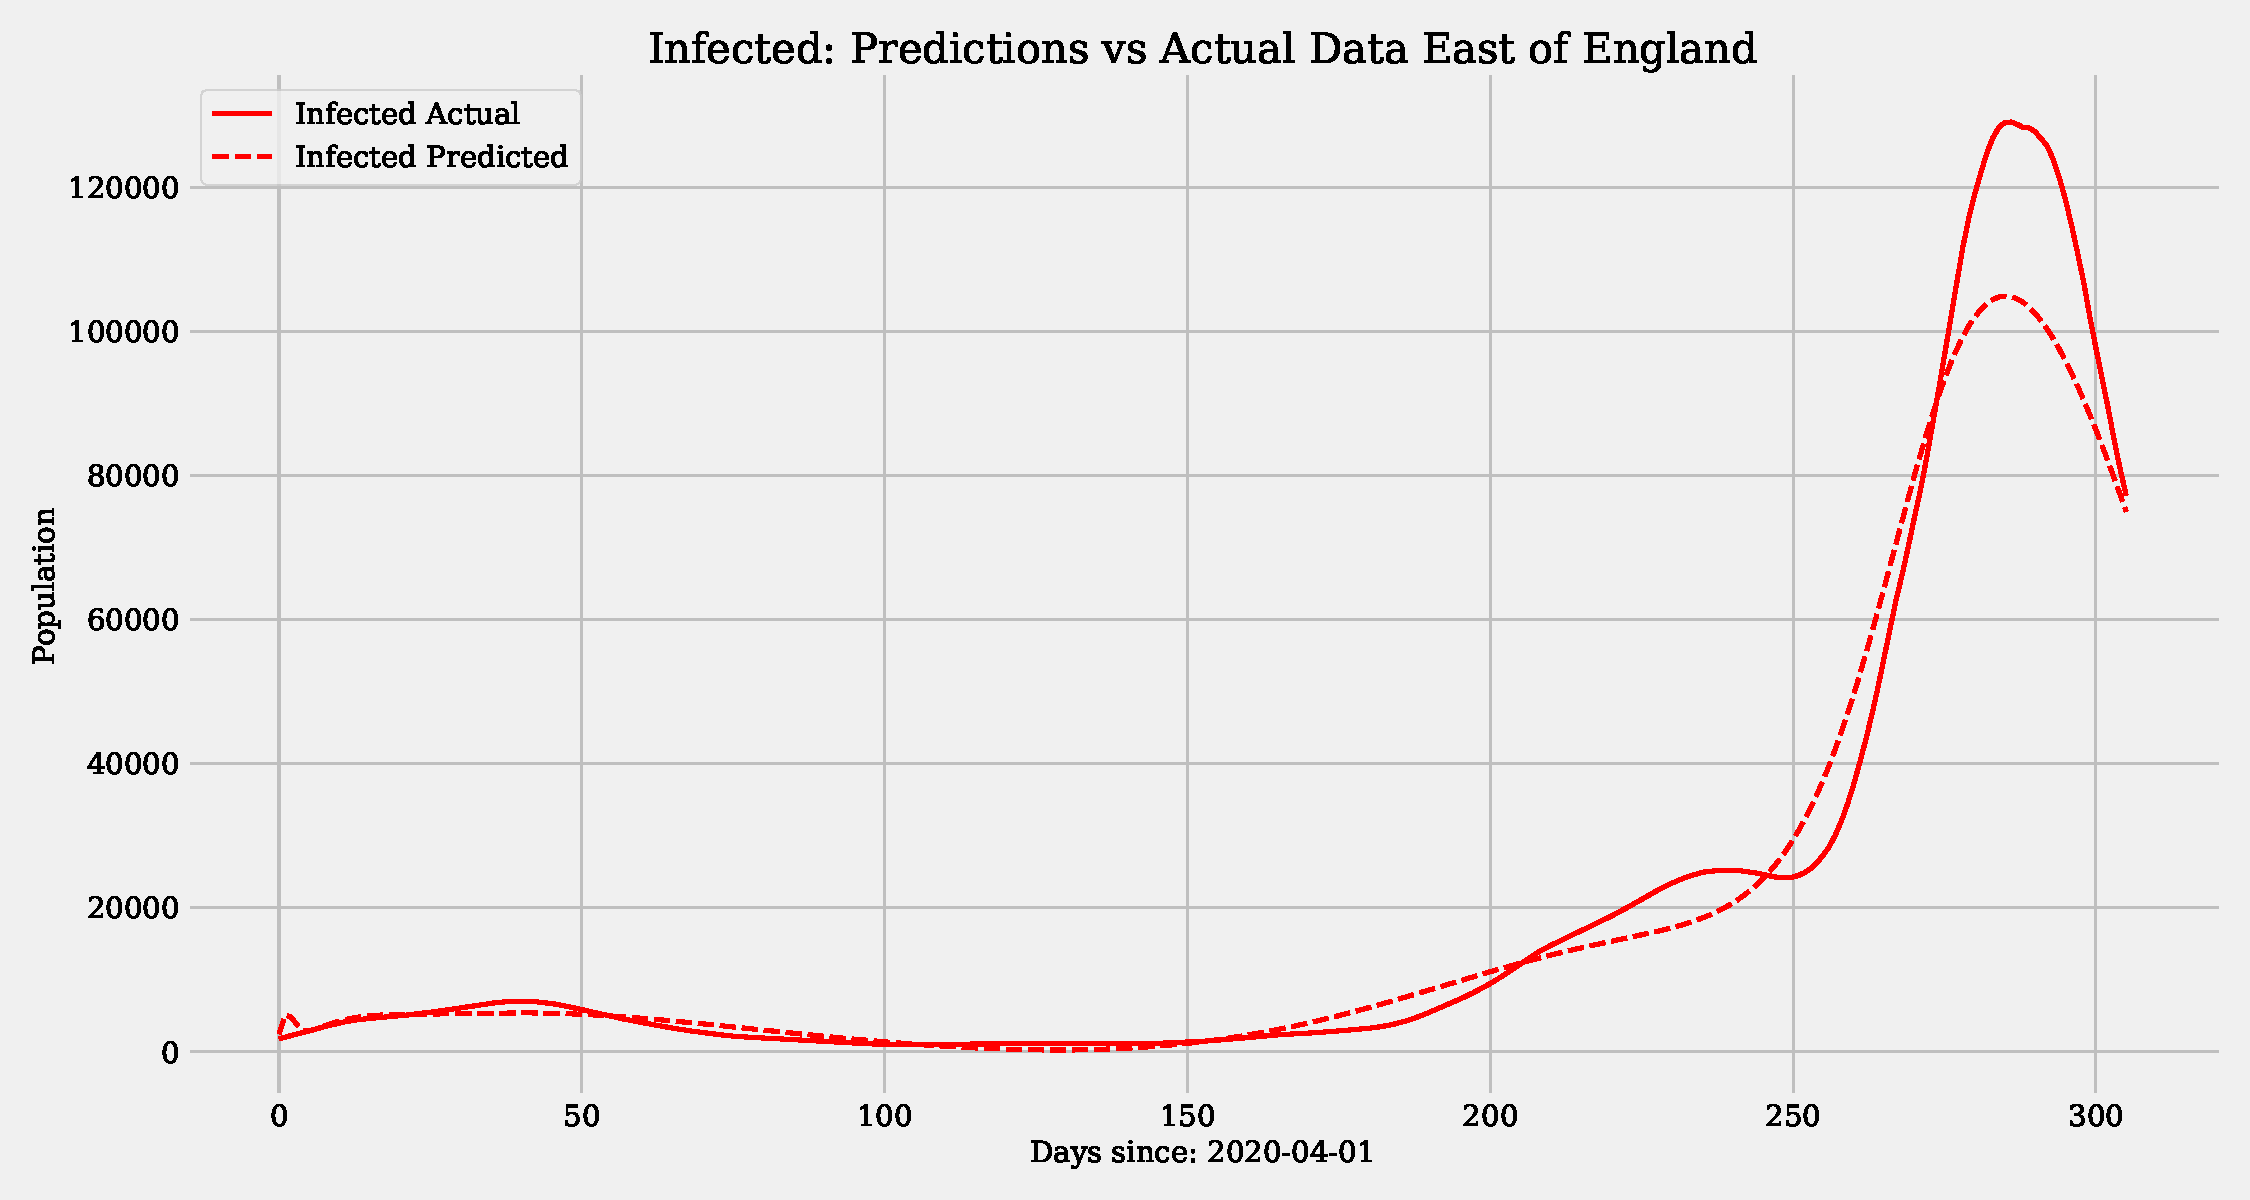
\includegraphics[width=0.8\textwidth]{images/pinn/I_predictions_East of England.pdf}
    \caption{Predicted number of infectious individuals in the East of England region.}
    \label{fig:I_predictions_East_of_England}
\end{figure*}

\begin{figure*}[ht]
    \centering
    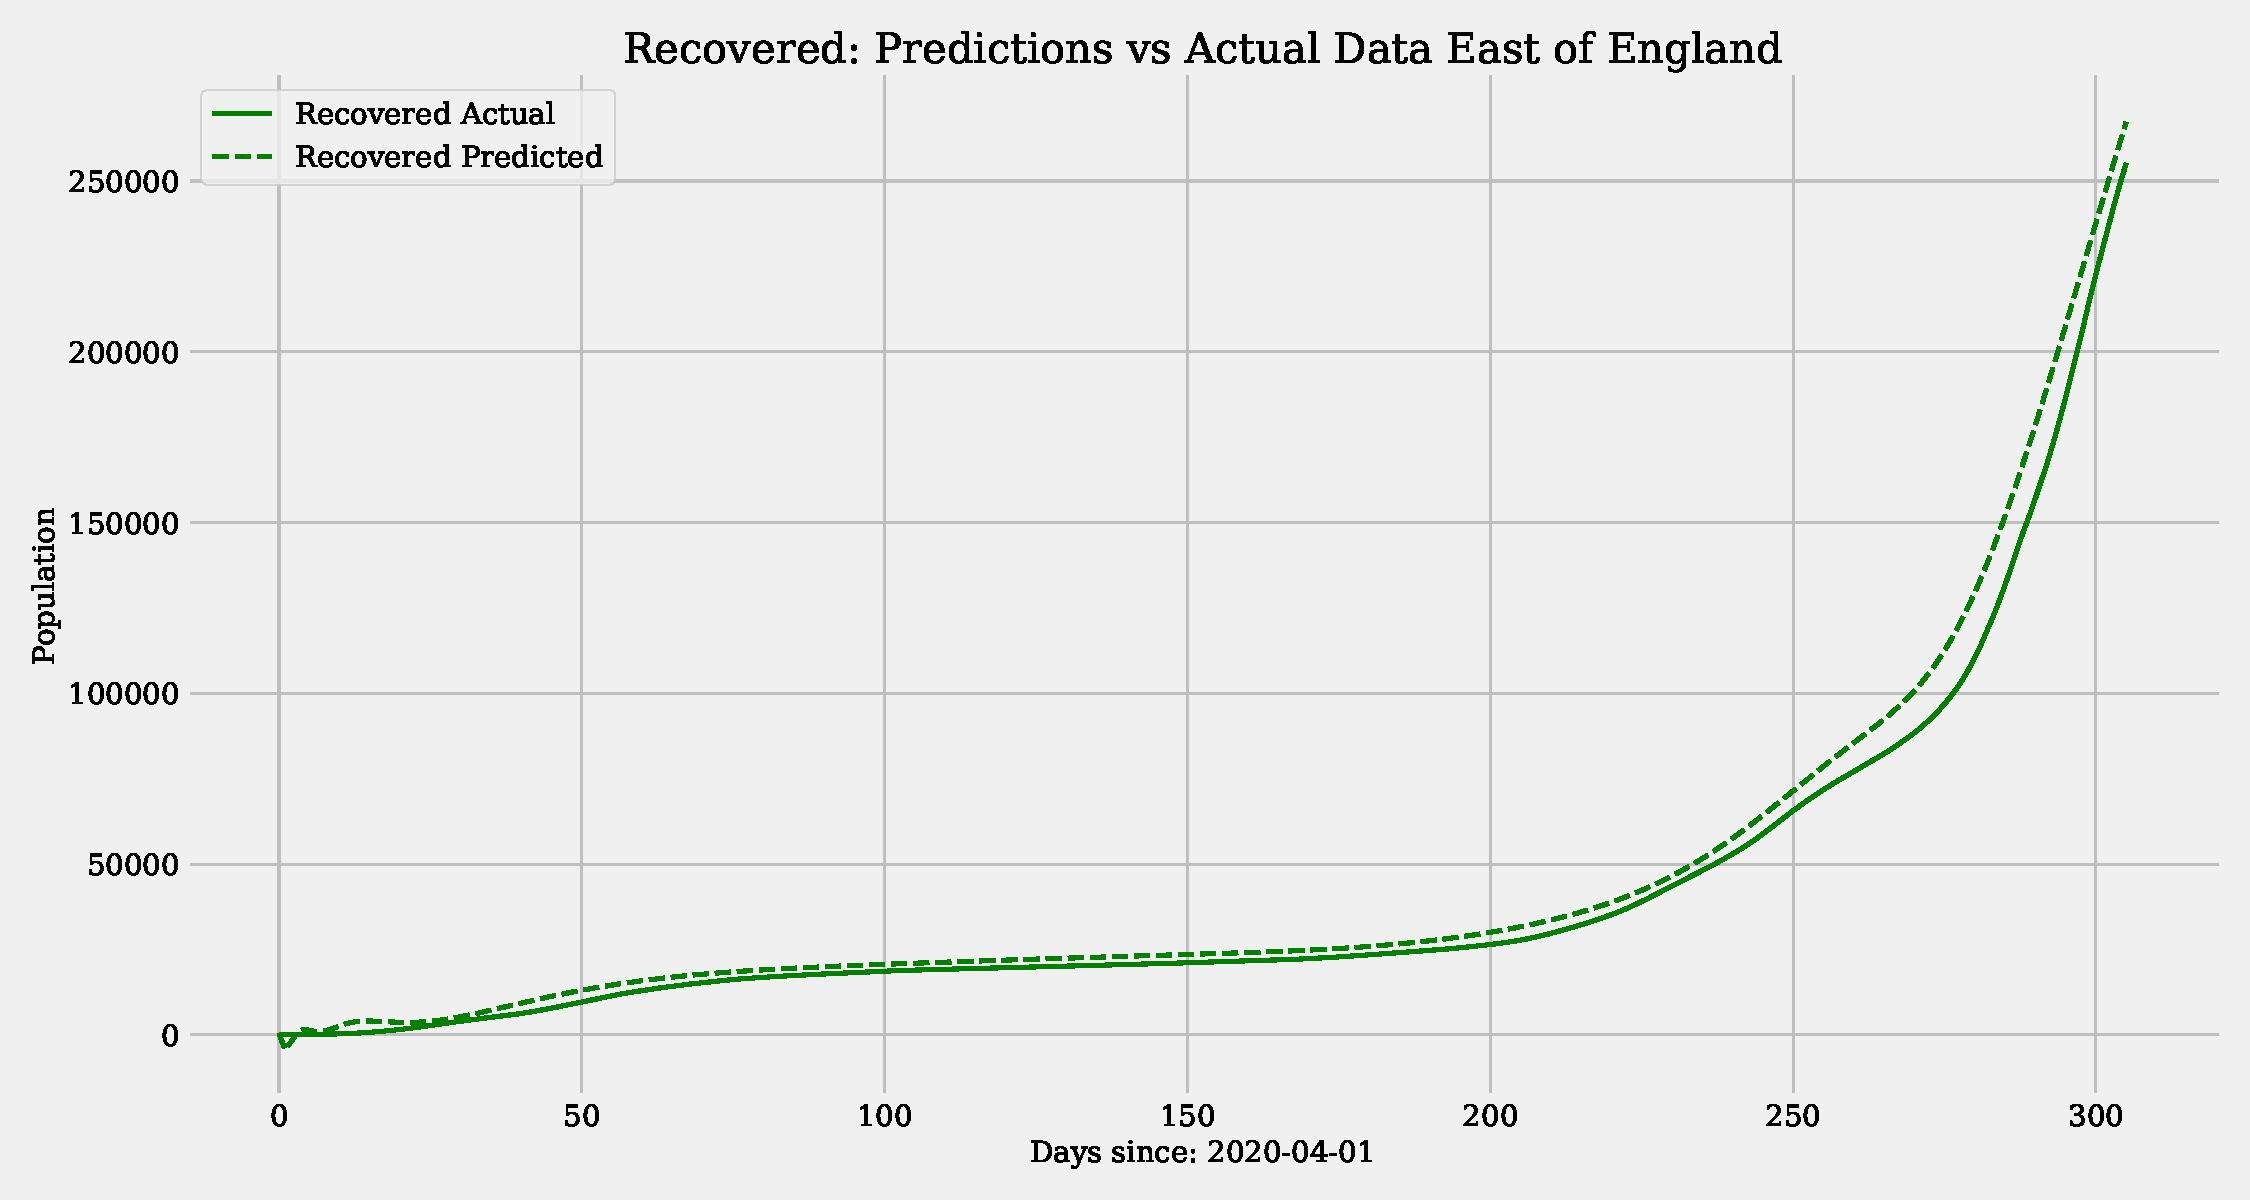
\includegraphics[width=0.8\textwidth]{images/pinn/R_predictions_East of England.pdf}
    \caption{Predicted number of recovered individuals in the East of England region.}
    \label{fig:R_predictions_East_of_England}
\end{figure*}

\begin{figure*}[ht]
    \centering
    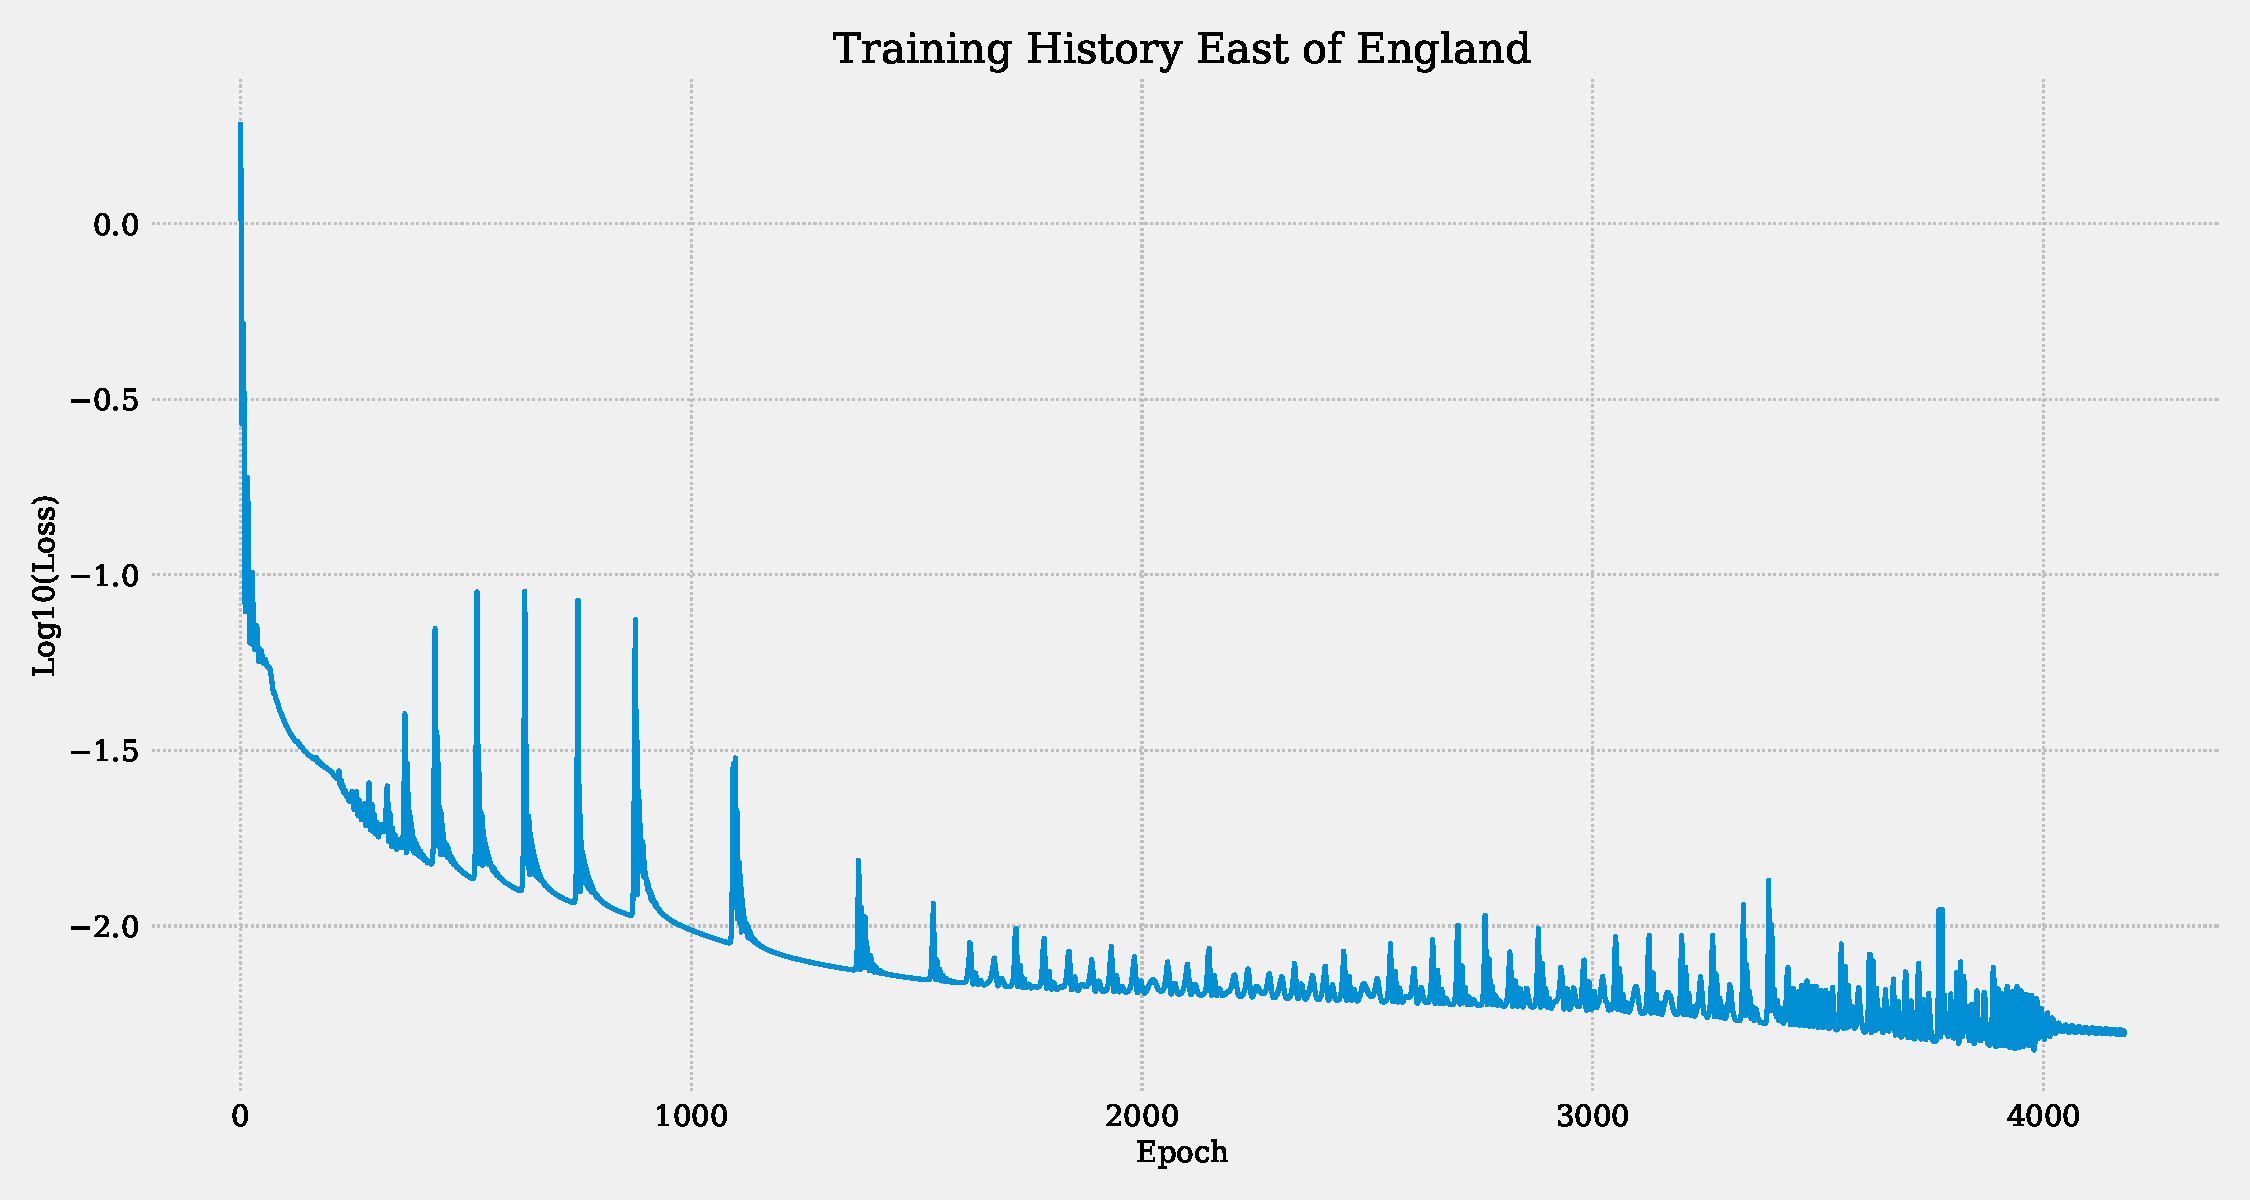
\includegraphics[width=0.8\textwidth]{images/pinn/Training_History_East of England.pdf}
    \caption{Training history of the PINN model for the East of England region.}
    \label{fig:Training_History_East_of_England}
\end{figure*}

\begin{figure*}[ht]
    \centering
    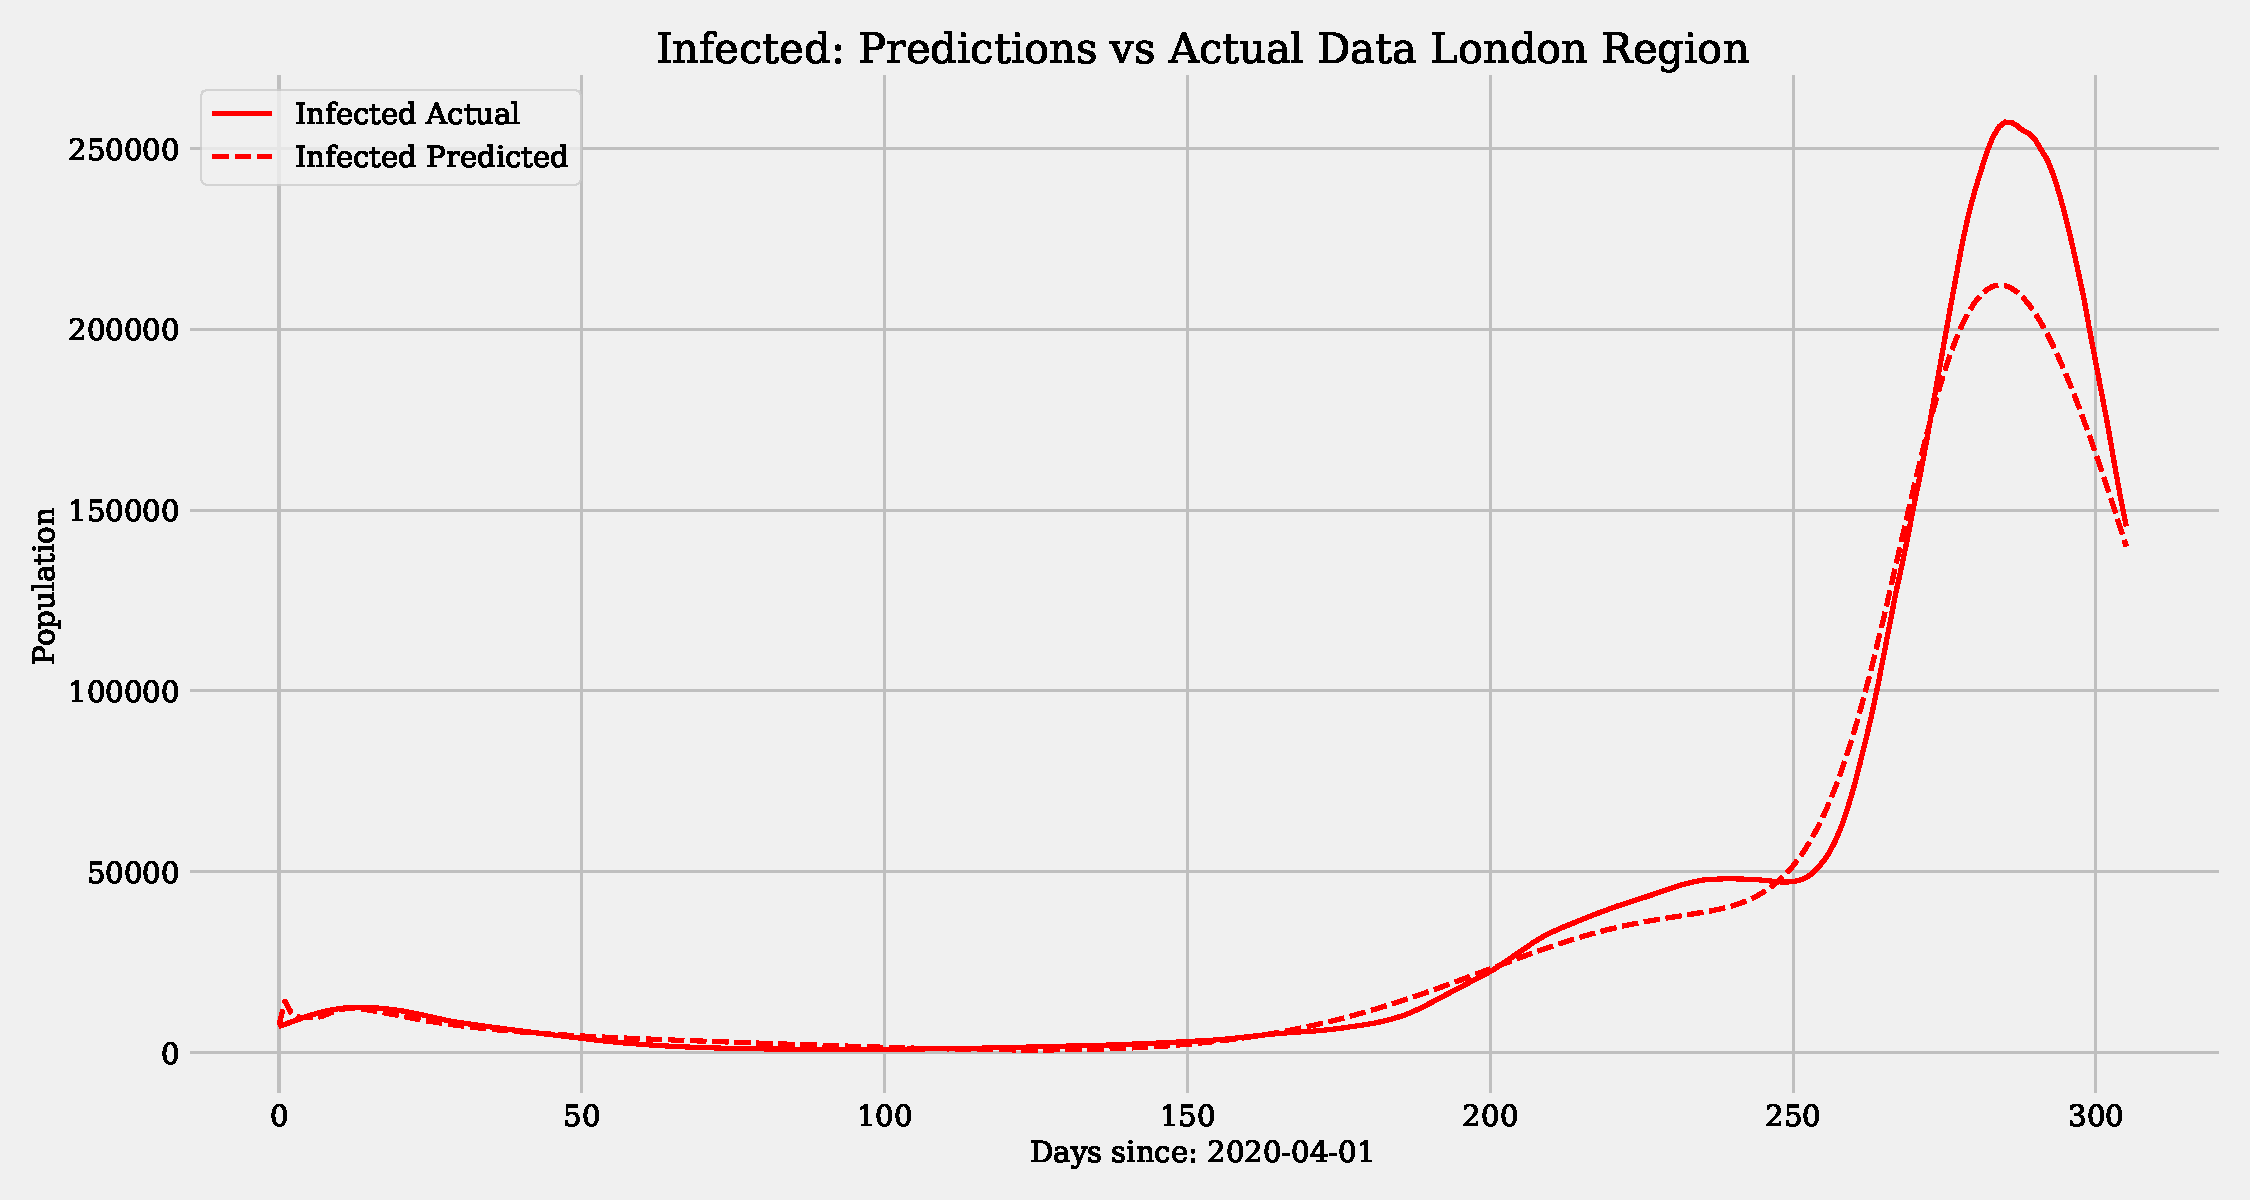
\includegraphics[width=0.8\textwidth]{images/pinn/I_predictions_London Region.pdf}
    \caption{Predicted number of infectious individuals in the London region.}
    \label{fig:I_predictions_London}
\end{figure*}

\begin{figure*}[ht]
    \centering
    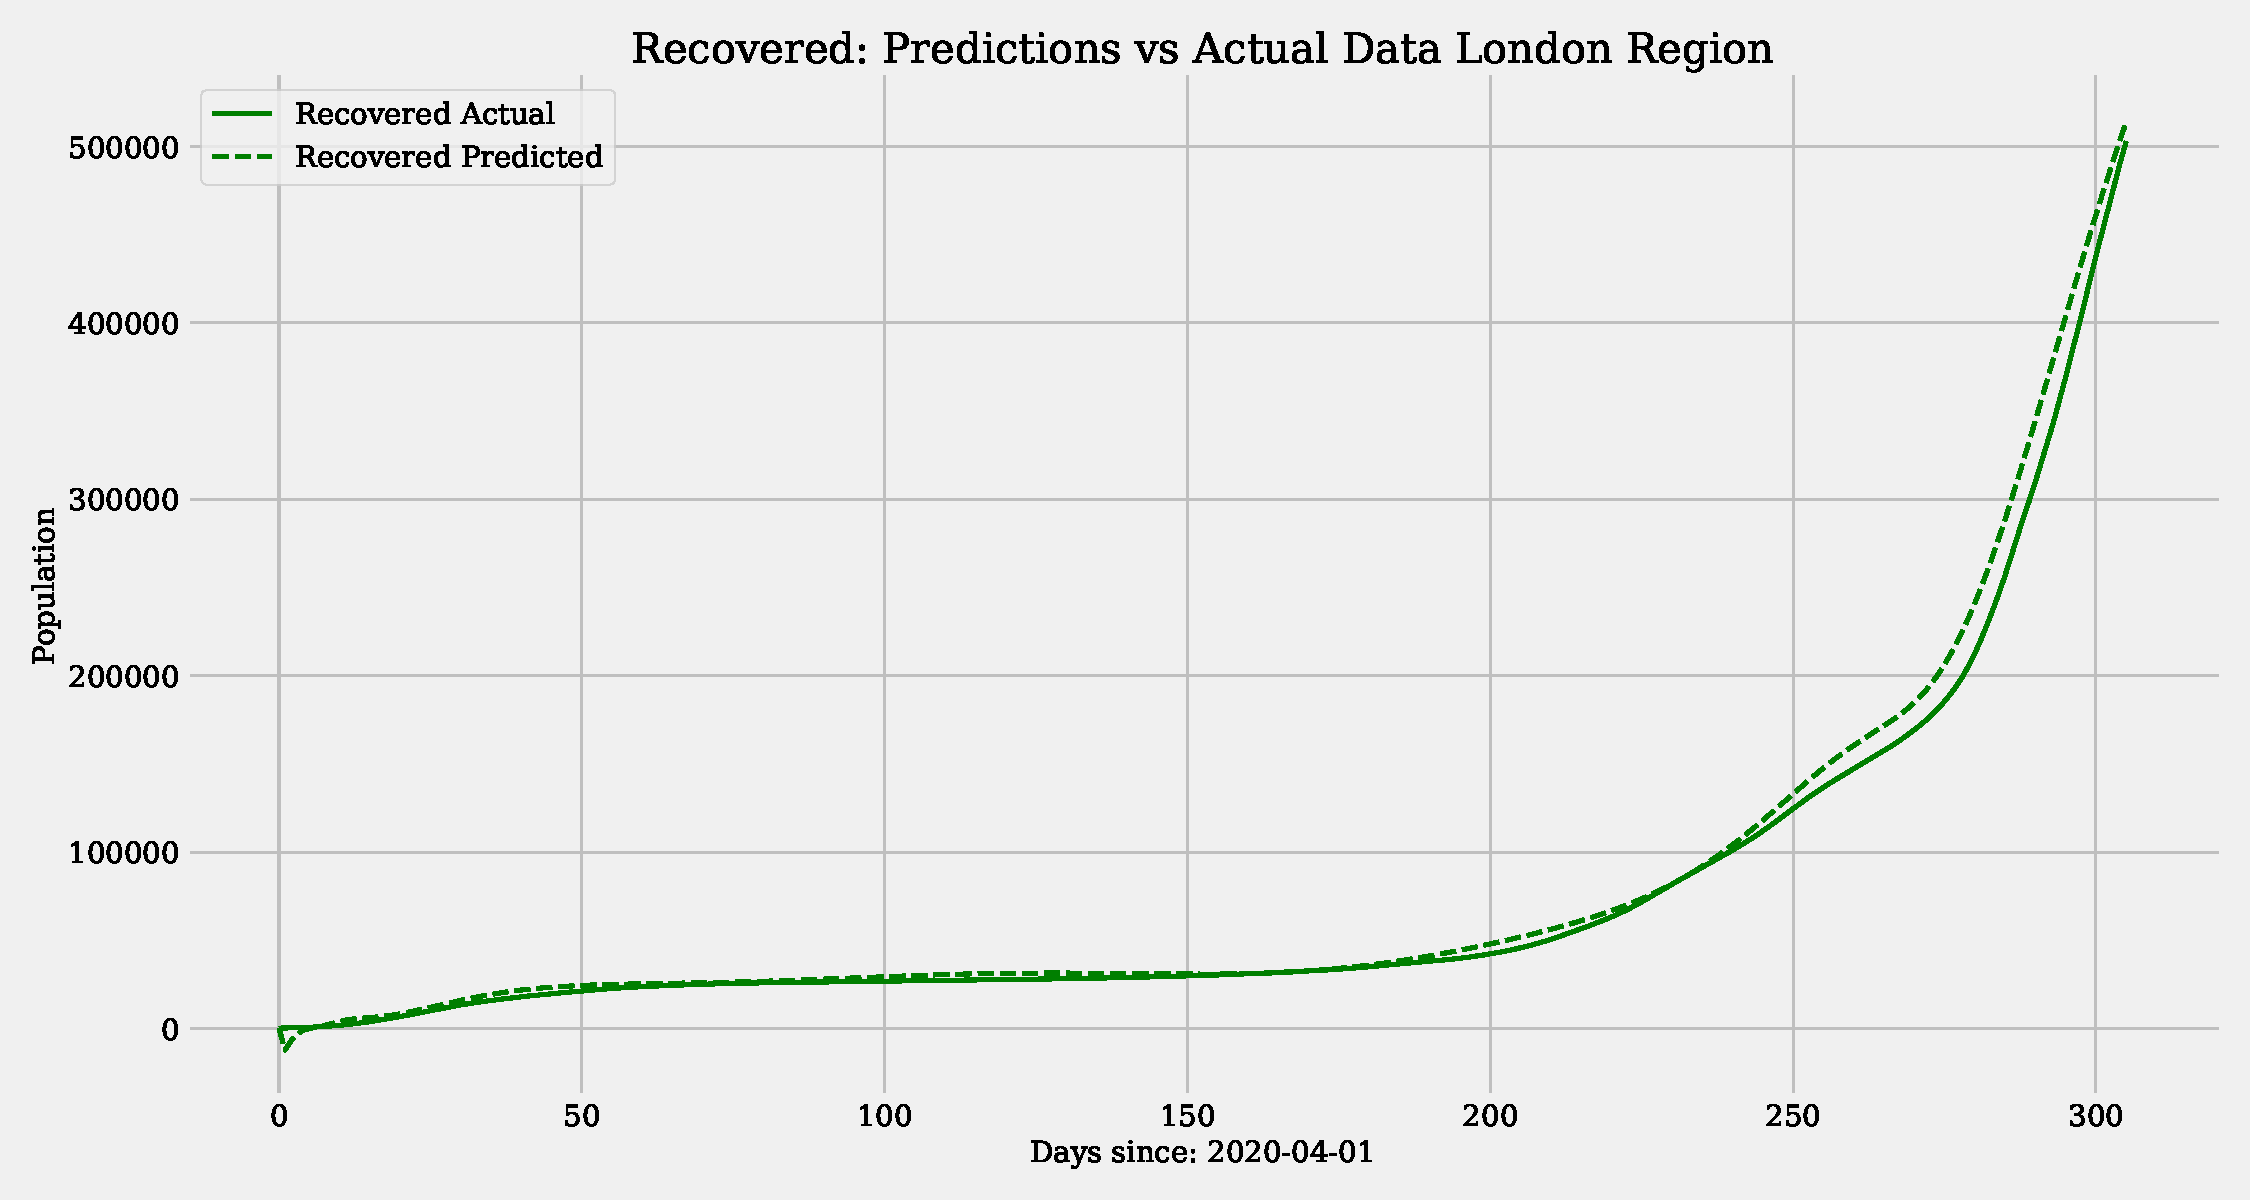
\includegraphics[width=0.8\textwidth]{images/pinn/R_predictions_London Region.pdf}
    \caption{Predicted number of recovered individuals in the London region.}
    \label{fig:R_predictions_London}
\end{figure*}

\begin{figure*}[ht]
    \centering
    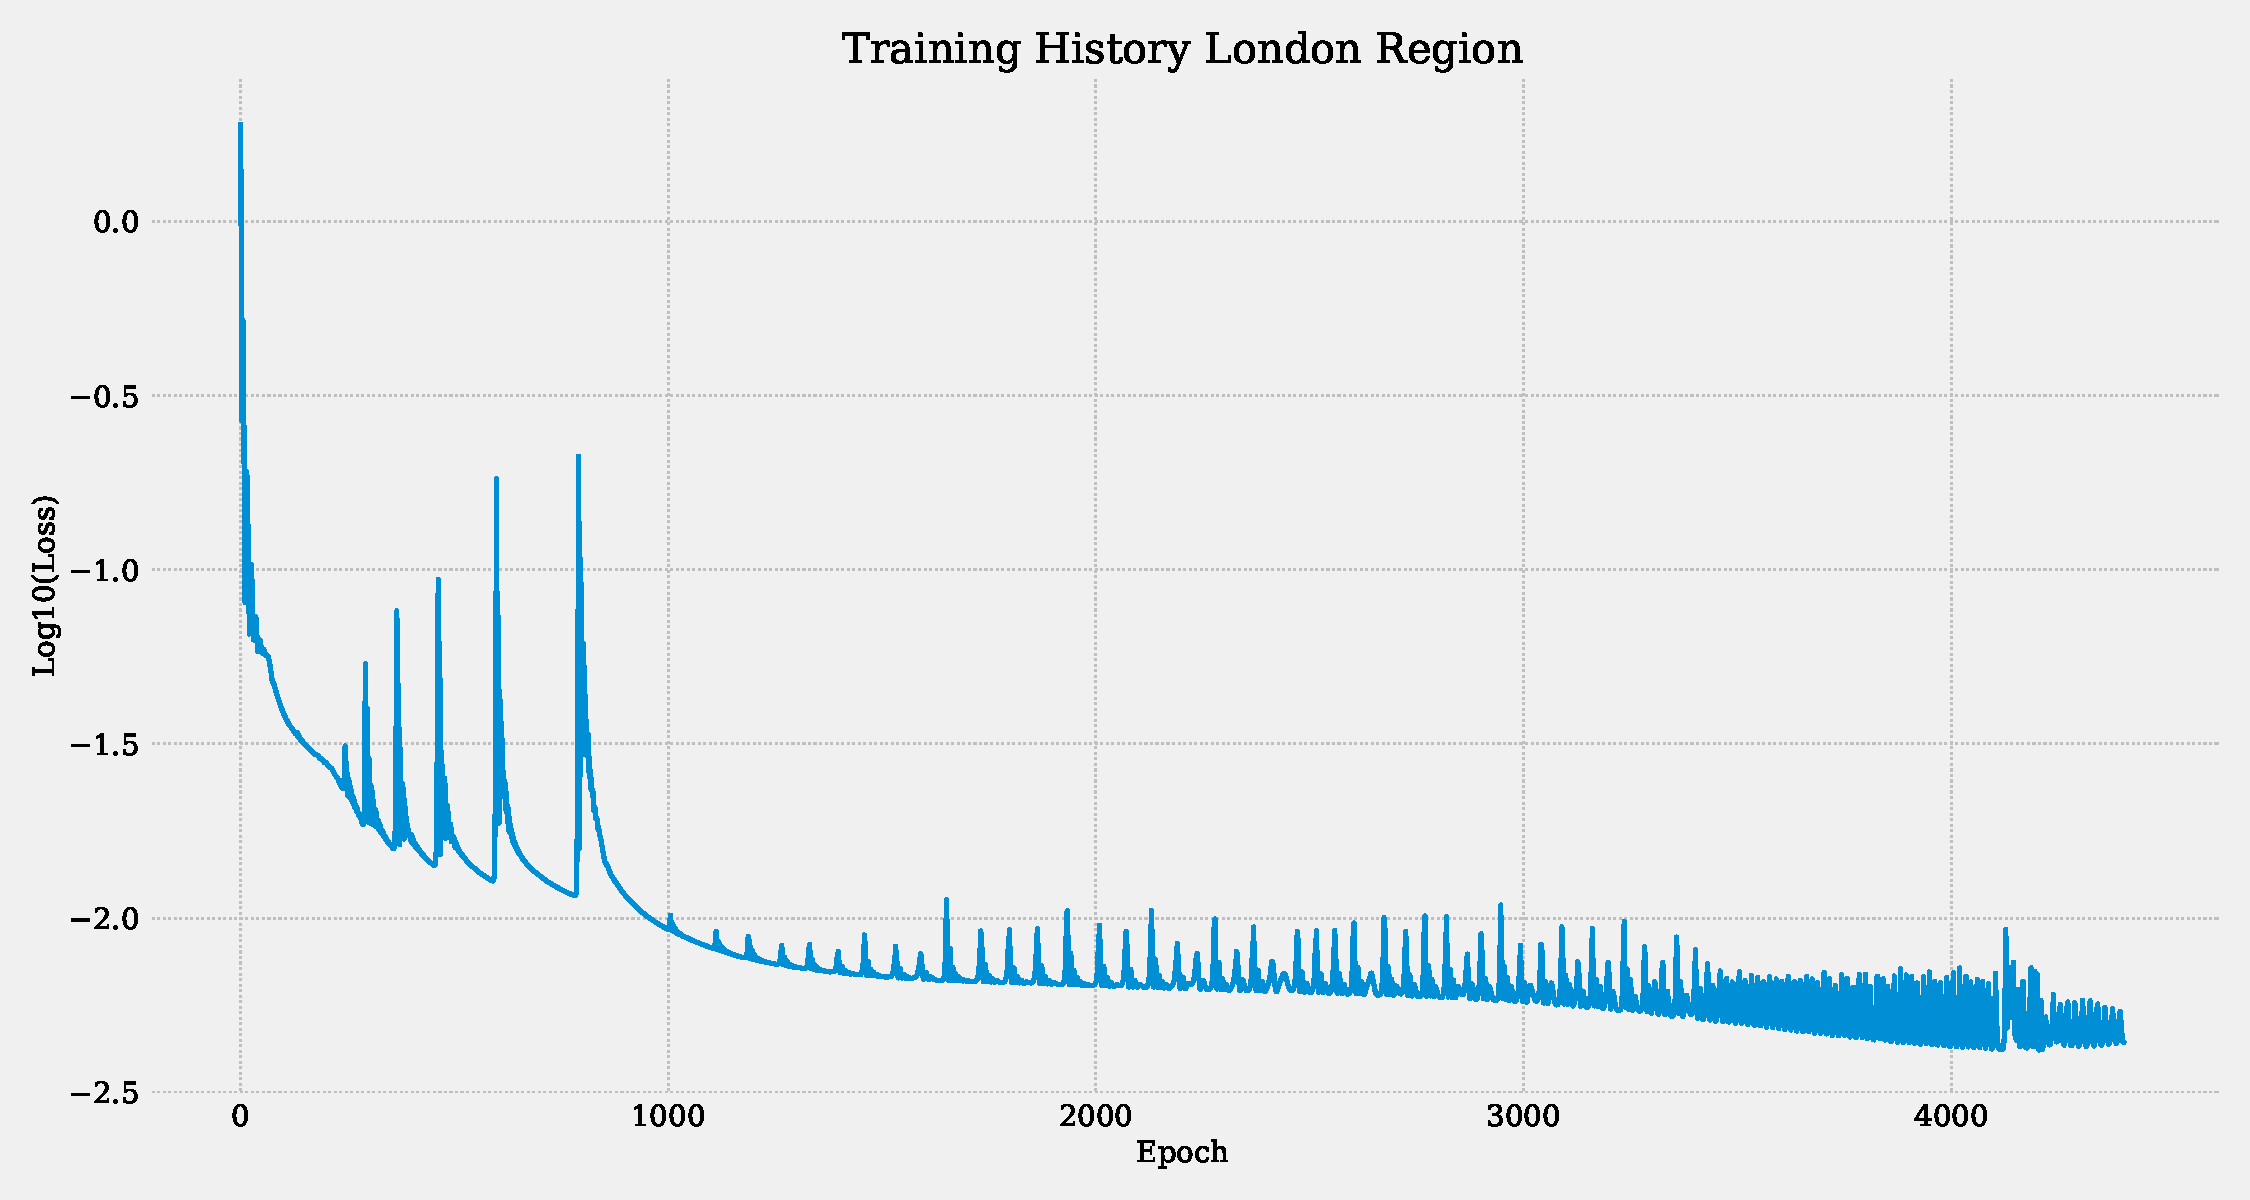
\includegraphics[width=0.8\textwidth]{images/pinn/Training_History_London Region.pdf}
    \caption{Training history of the PINN model for the London region.}
    \label{fig:Training_History_London}
\end{figure*}


\bibliographystyle{alphaurl}
\bibliography{refs}
\end{document}